\chapter{Instrumentos de medición}
Todas las fotografías que se encuentran en esta sección, corresponden a los instrumentos que se encuentran en el laboratorio de mediciones de la EETP669.
\section{Galvanómetro}
\section{Multímetro}

\begin{figure}[htbp]
  \centering
  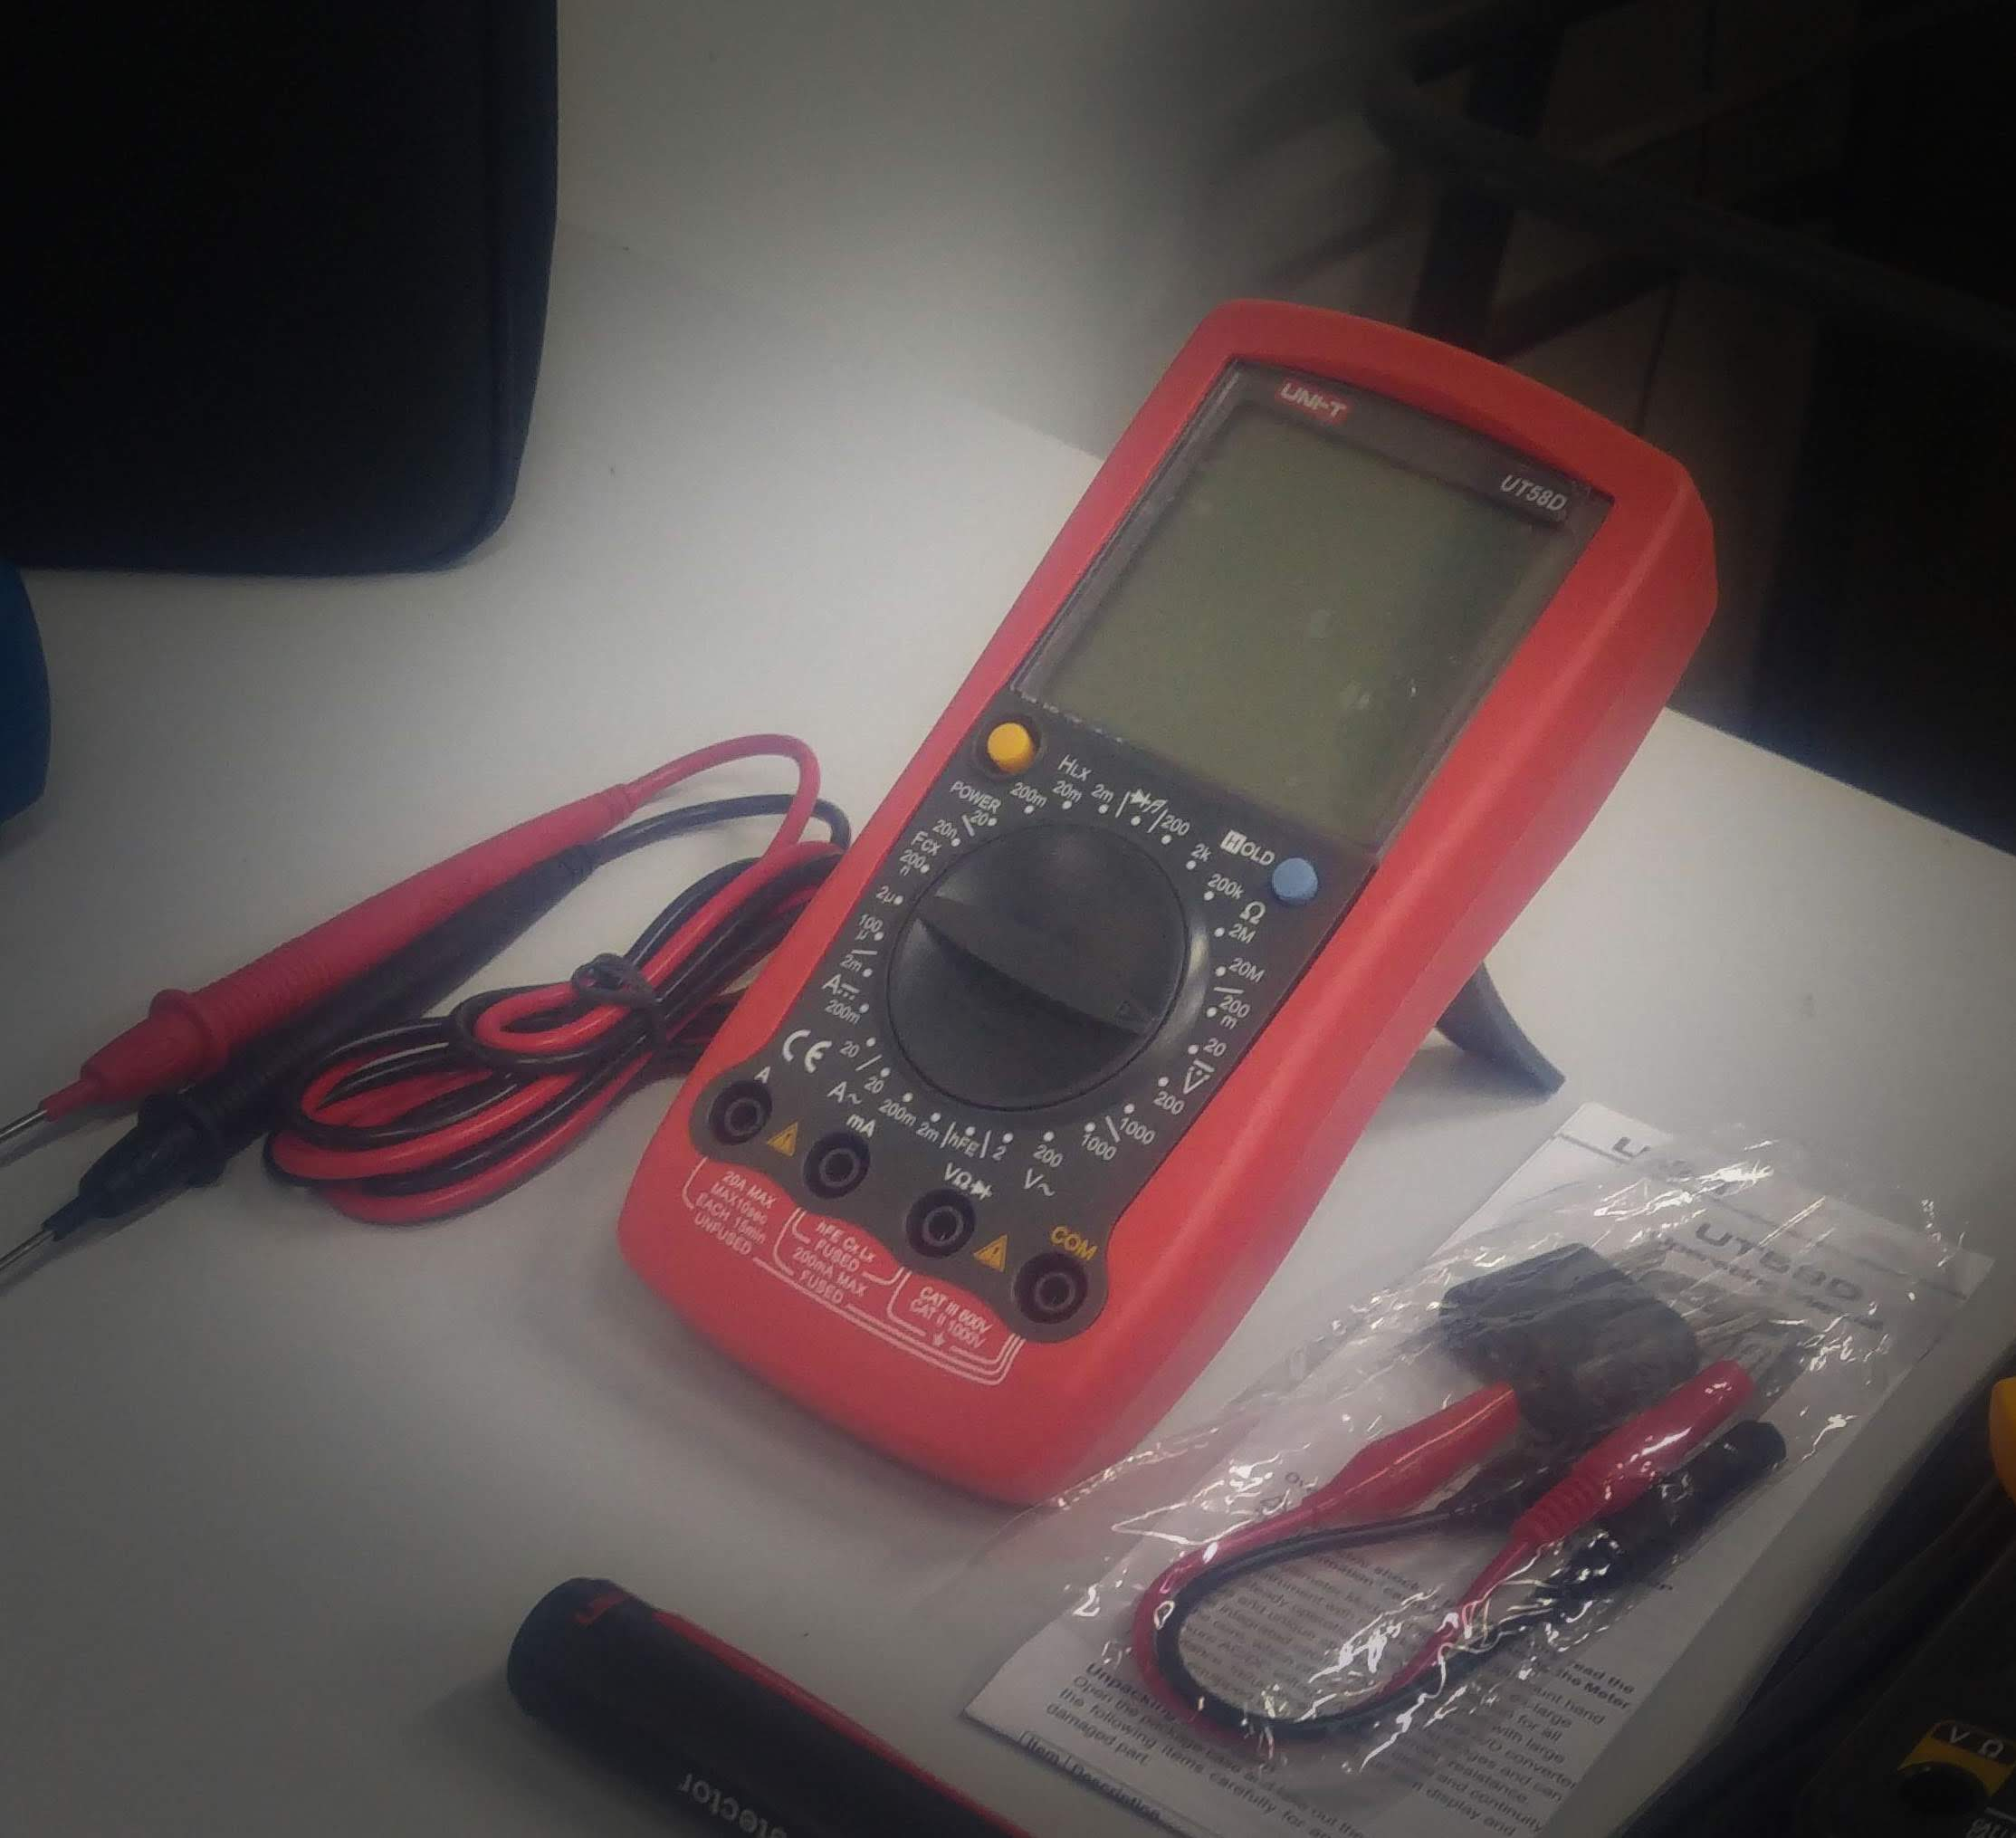
\includegraphics[width=0.5\textwidth]{images/fotos/tester1.jpg}
  \caption{Multímetro}
  \label{fig:multimetro_1}
\end{figure}

\begin{figure}[htbp]
  \centering  
  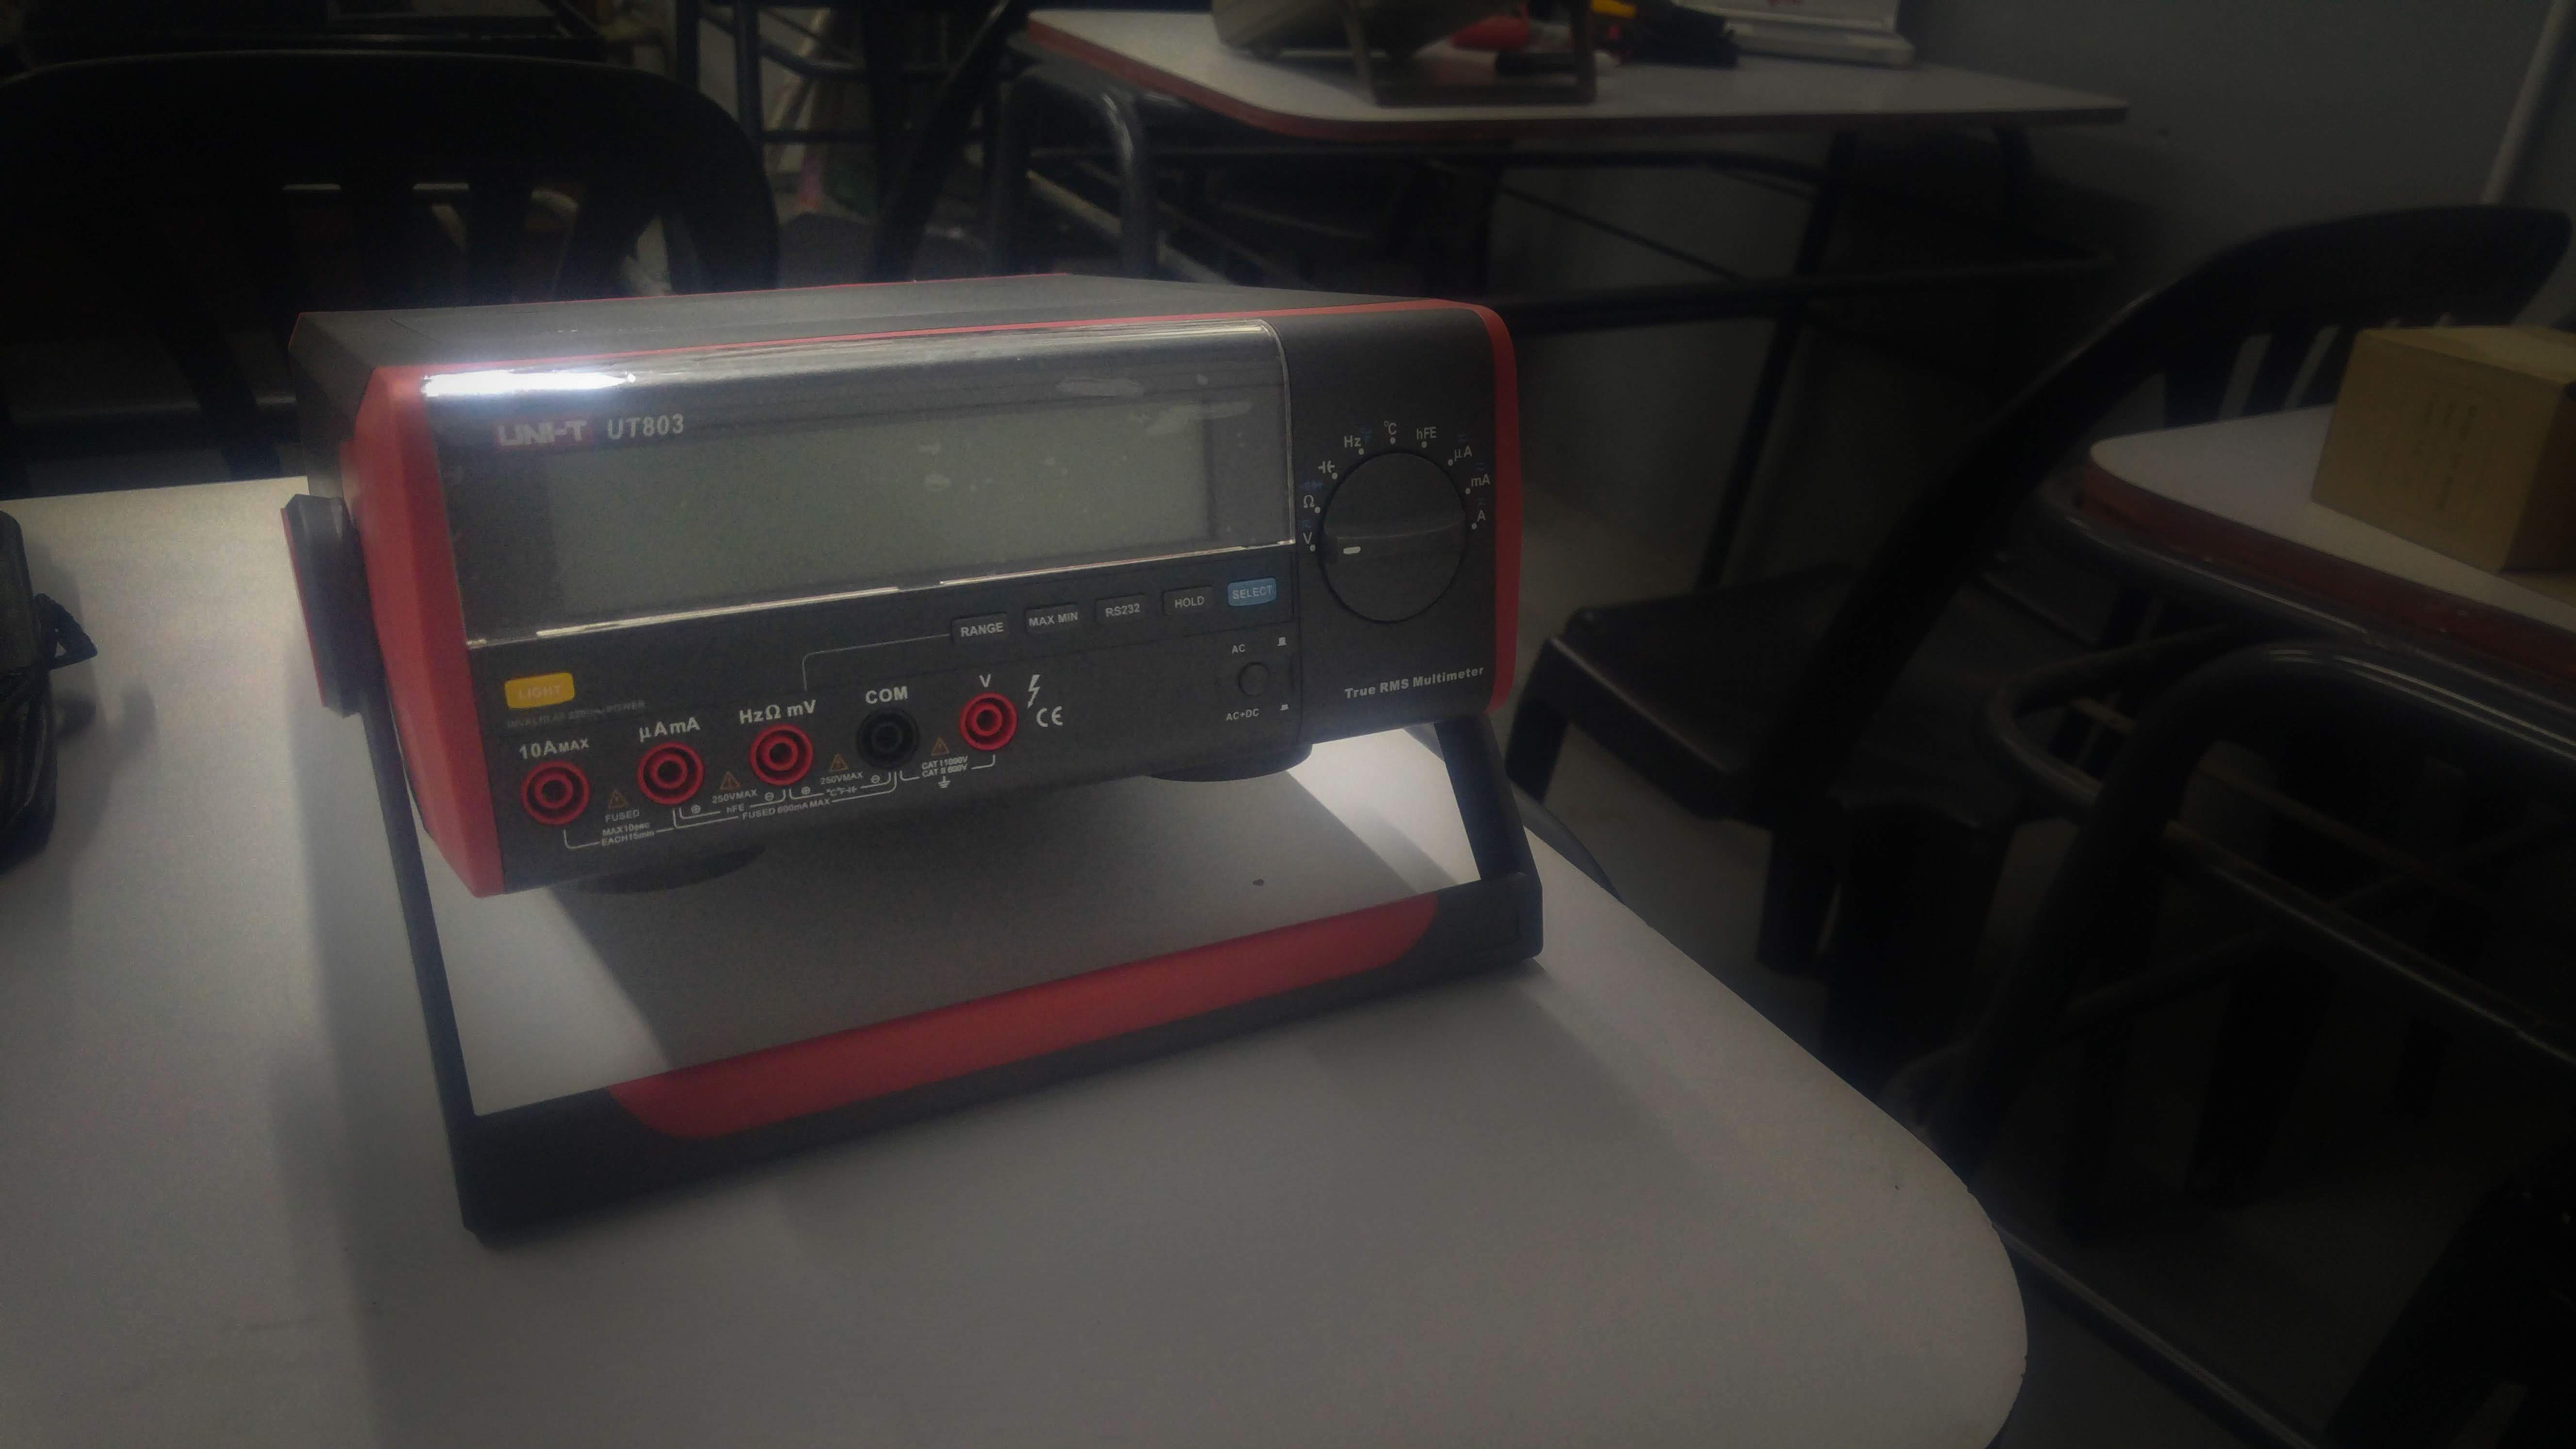
\includegraphics[width=0.5\textwidth]{images/fotos/testerdebanco.jpg}
  \caption{Multímetro de banco}
  \label{fig:multimetro_banco}
\end{figure}

\begin{figure}[htbp]
  \centering
  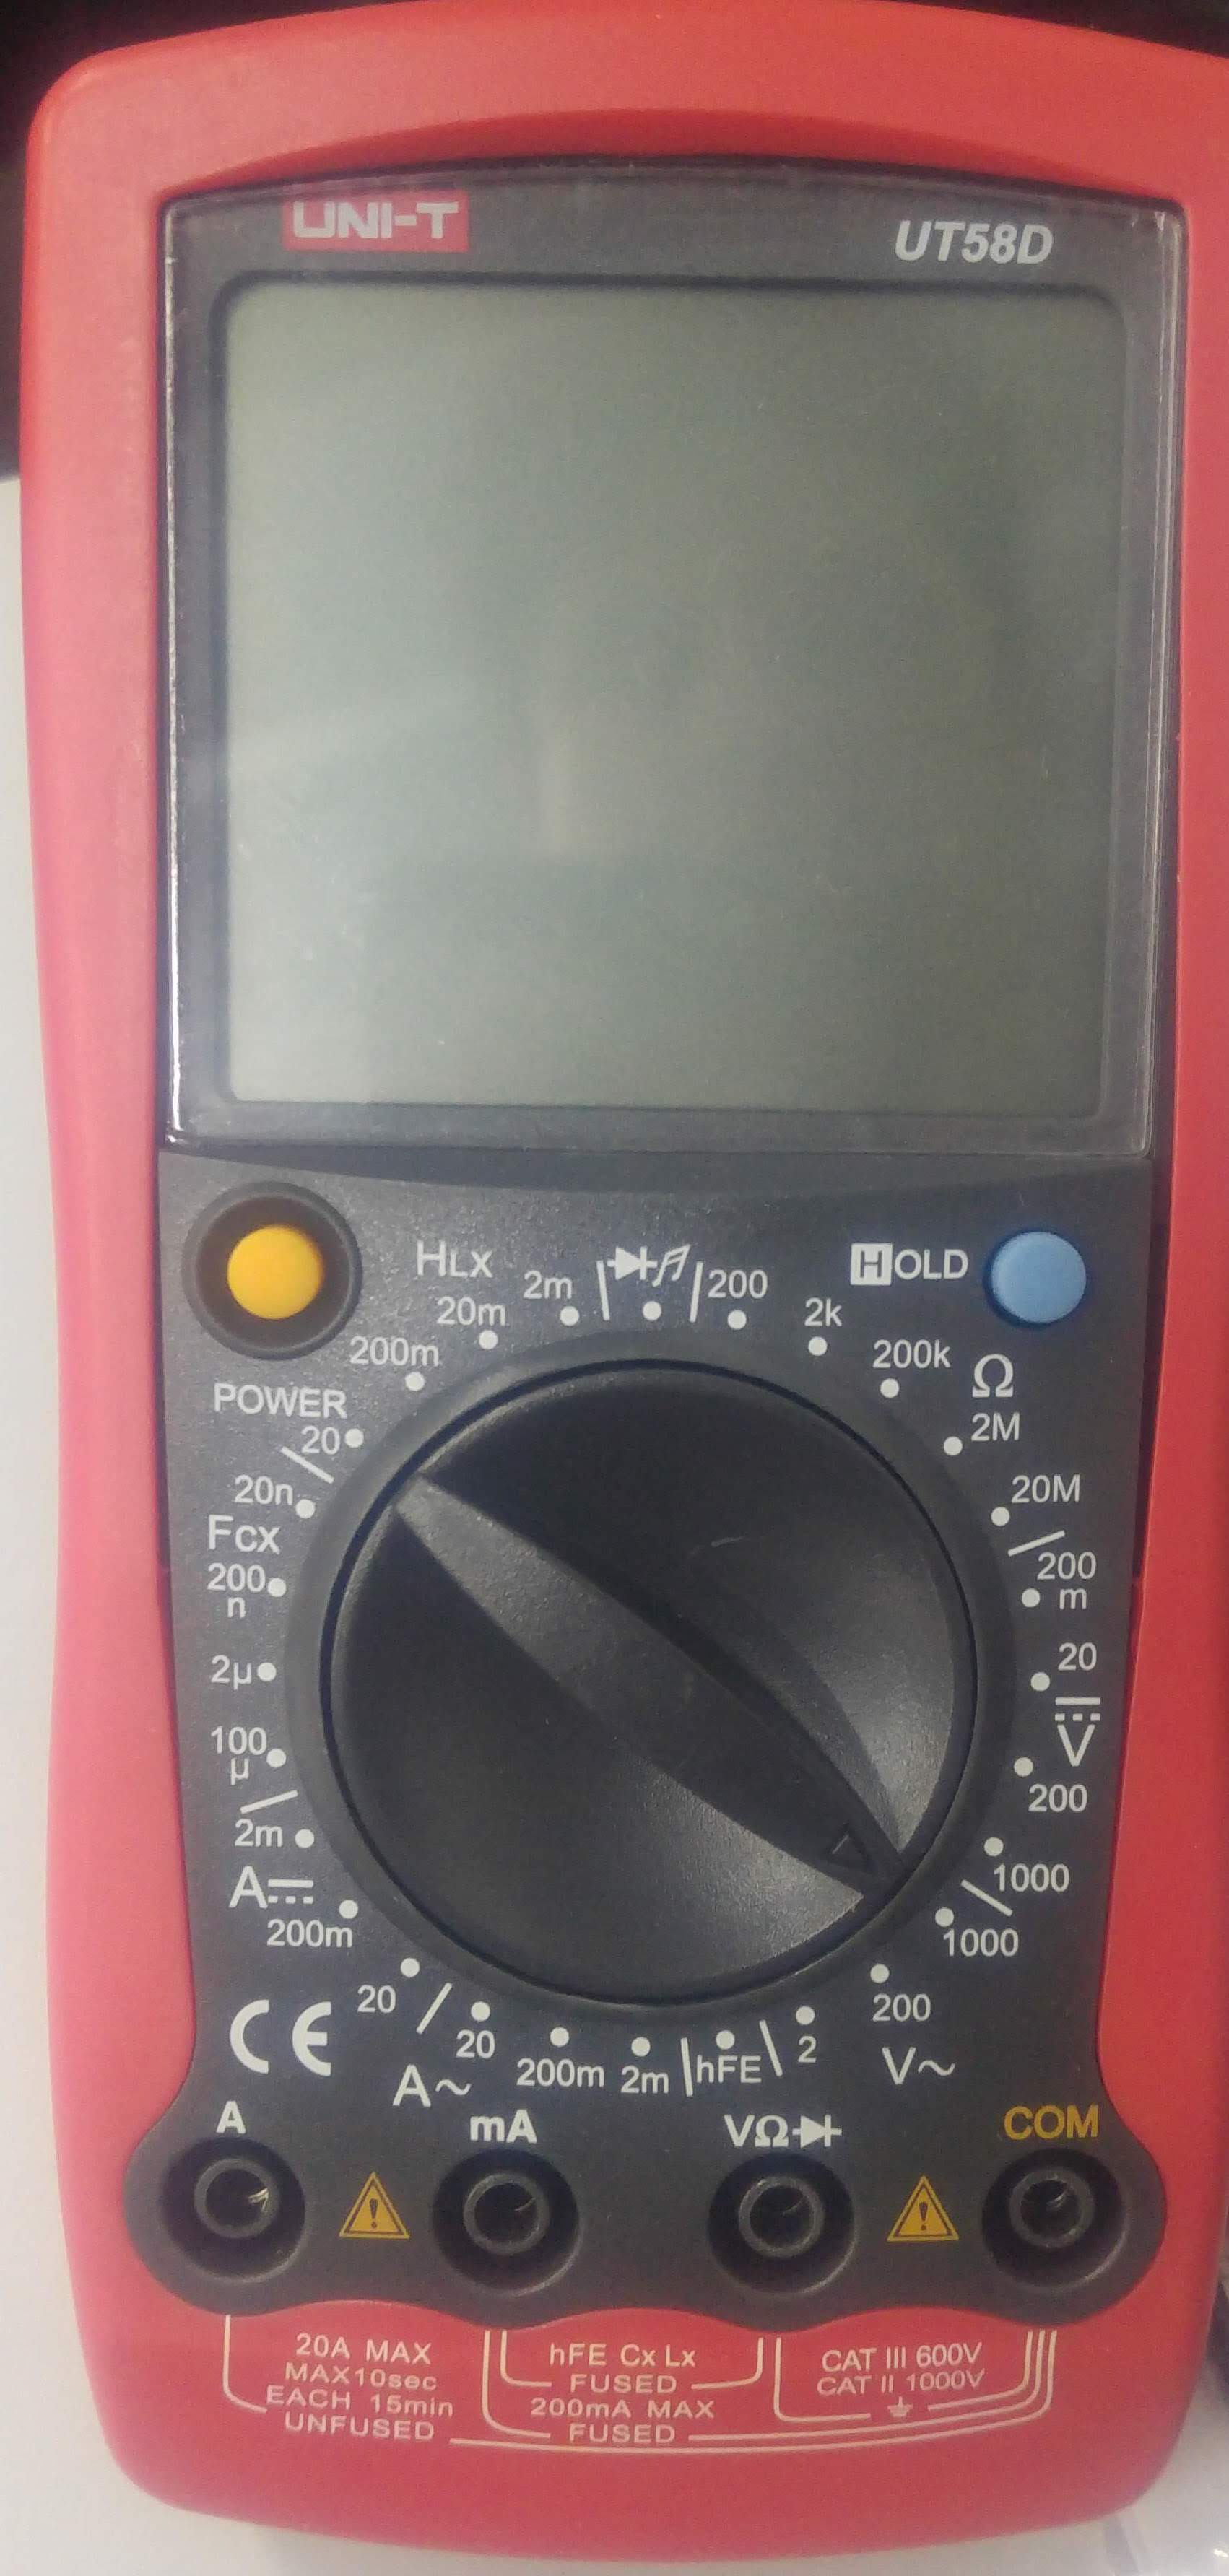
\includegraphics[width=\textwidth,height=\textheight,keepaspectratio]{images/fotos/tester3.jpg}
  \caption{Vista frontal de multímetro digital}
  \label{fig:multimetro_frente}
\end{figure}
\subsection{Voltímetro}
\begin{figure}[htbp]
  \centering  
  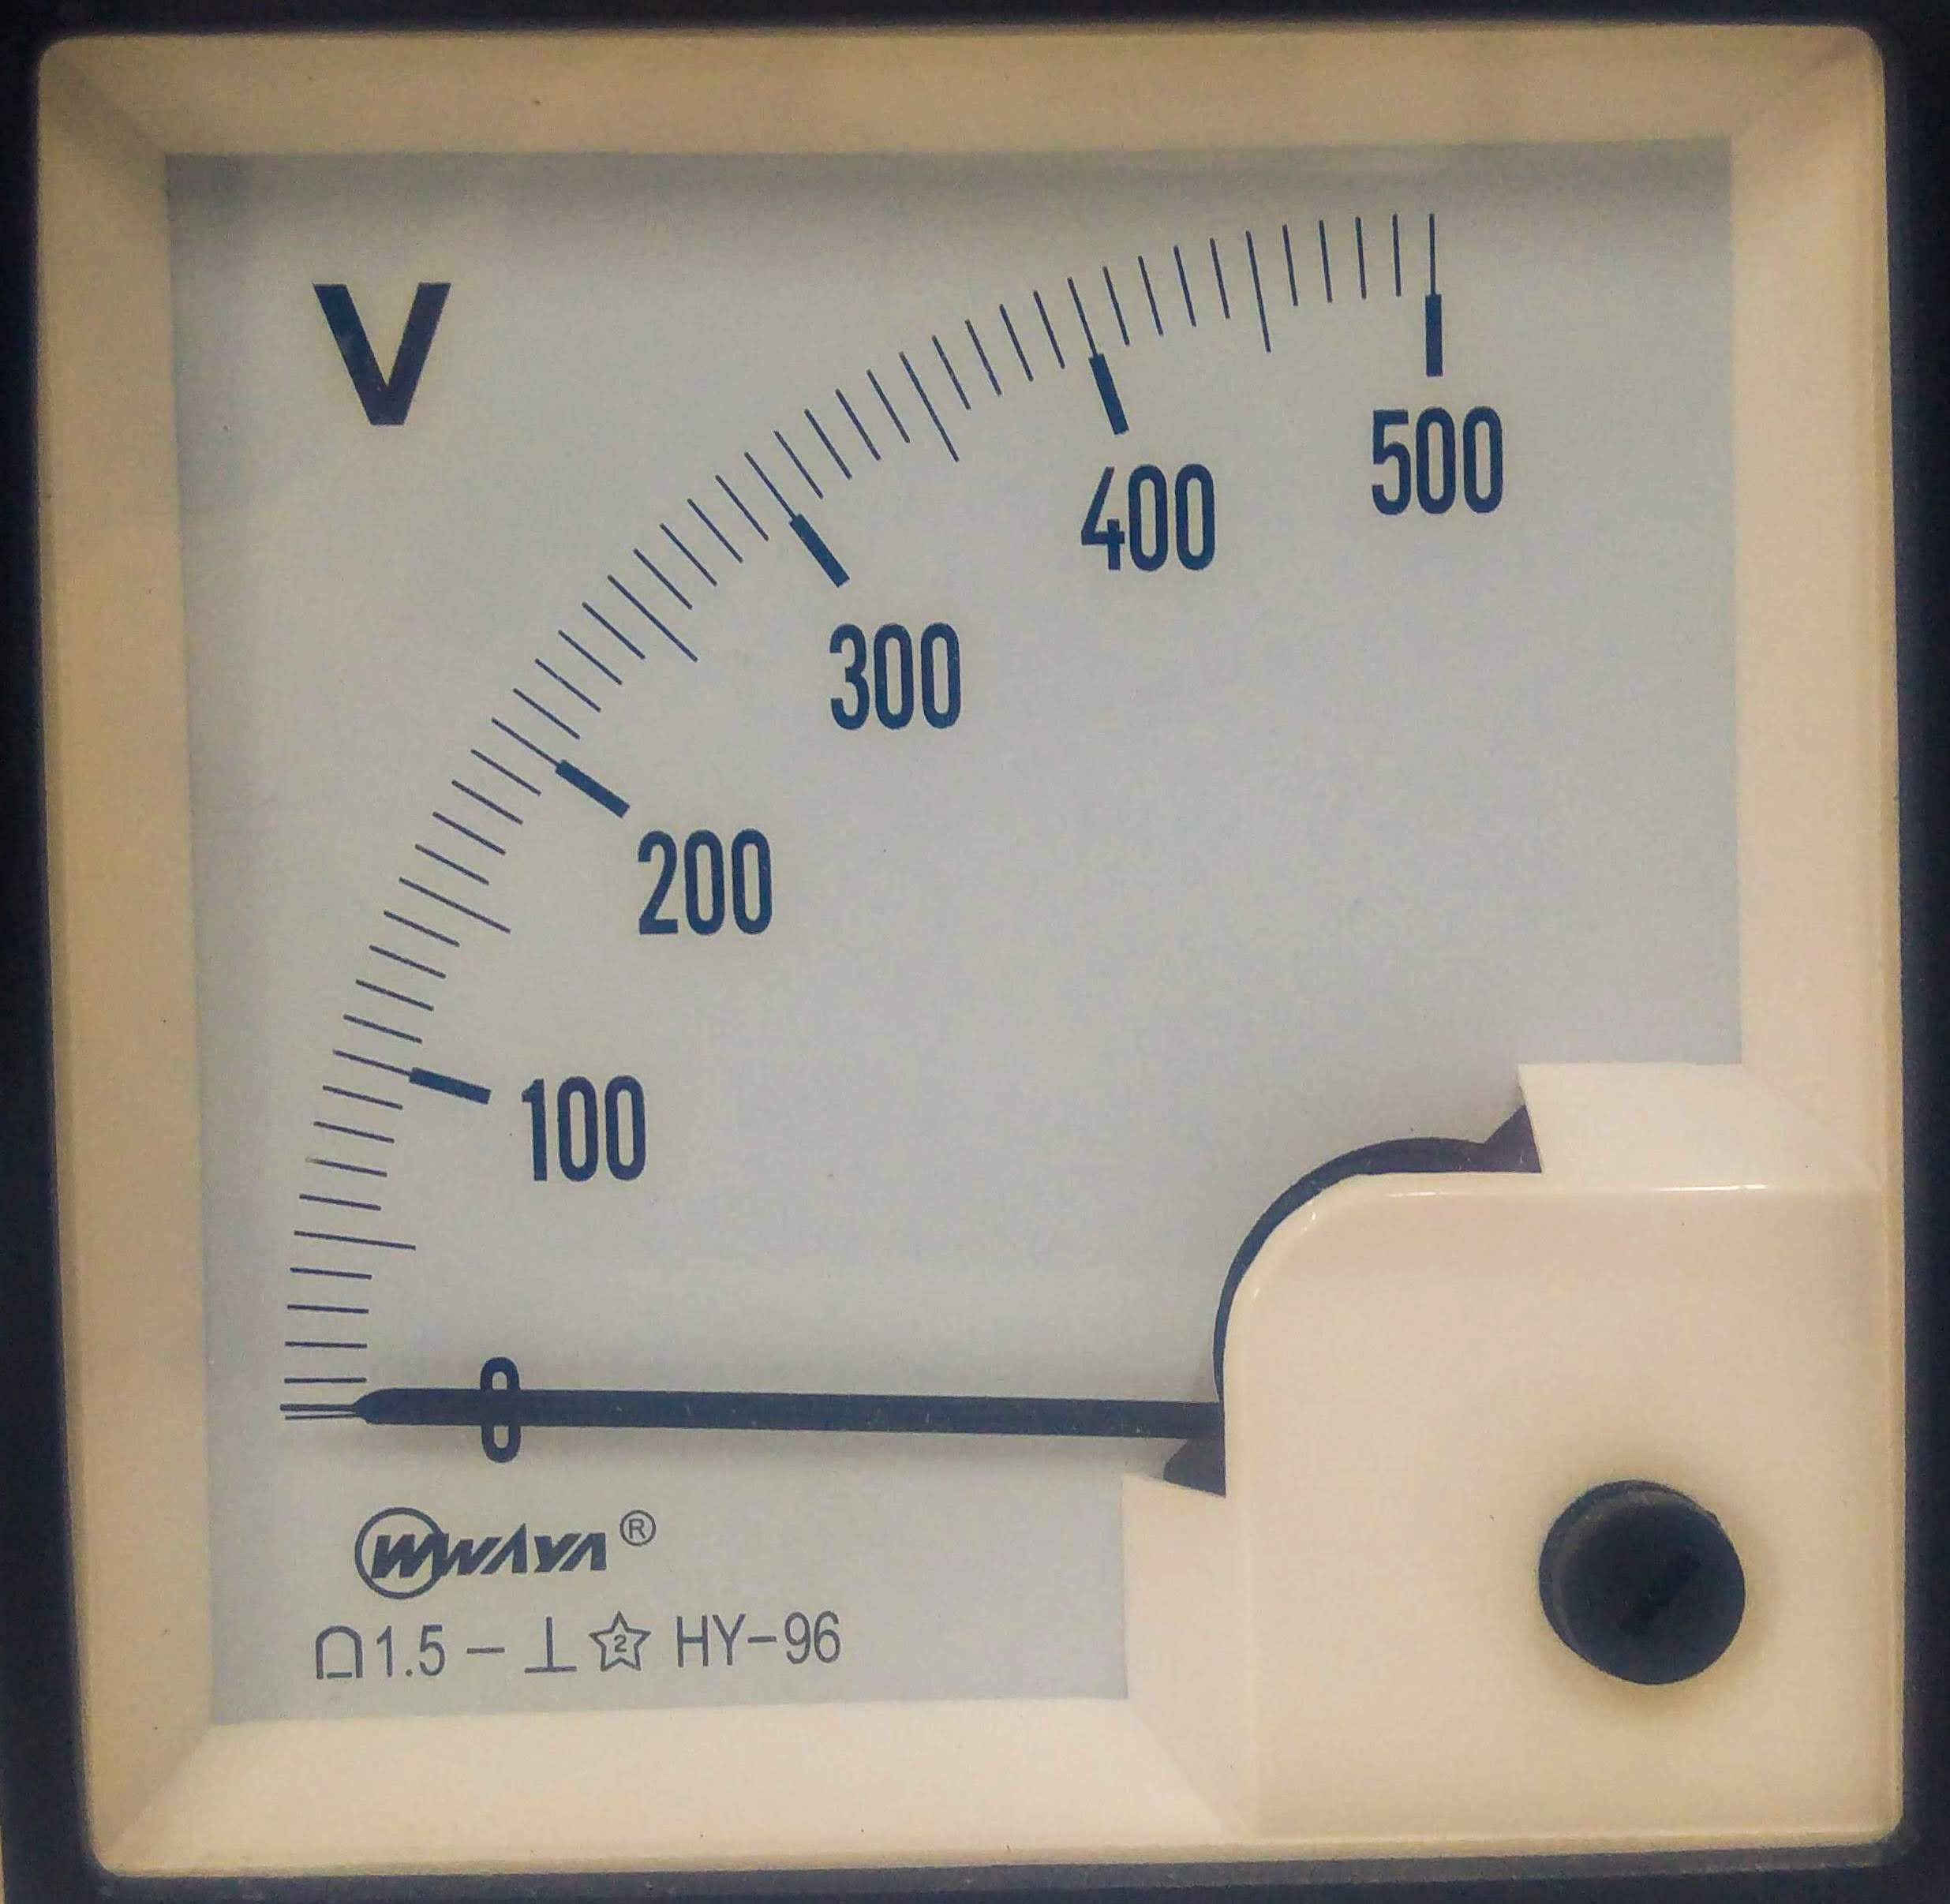
\includegraphics[width=0.5\textwidth]{images/fotos/voltimetro.jpg}
  \caption{Voltímetro}
  \label{fig:voltimetro}
\end{figure}
\subsection{Amperímetro}

\begin{figure}[htbp]
  \centering
  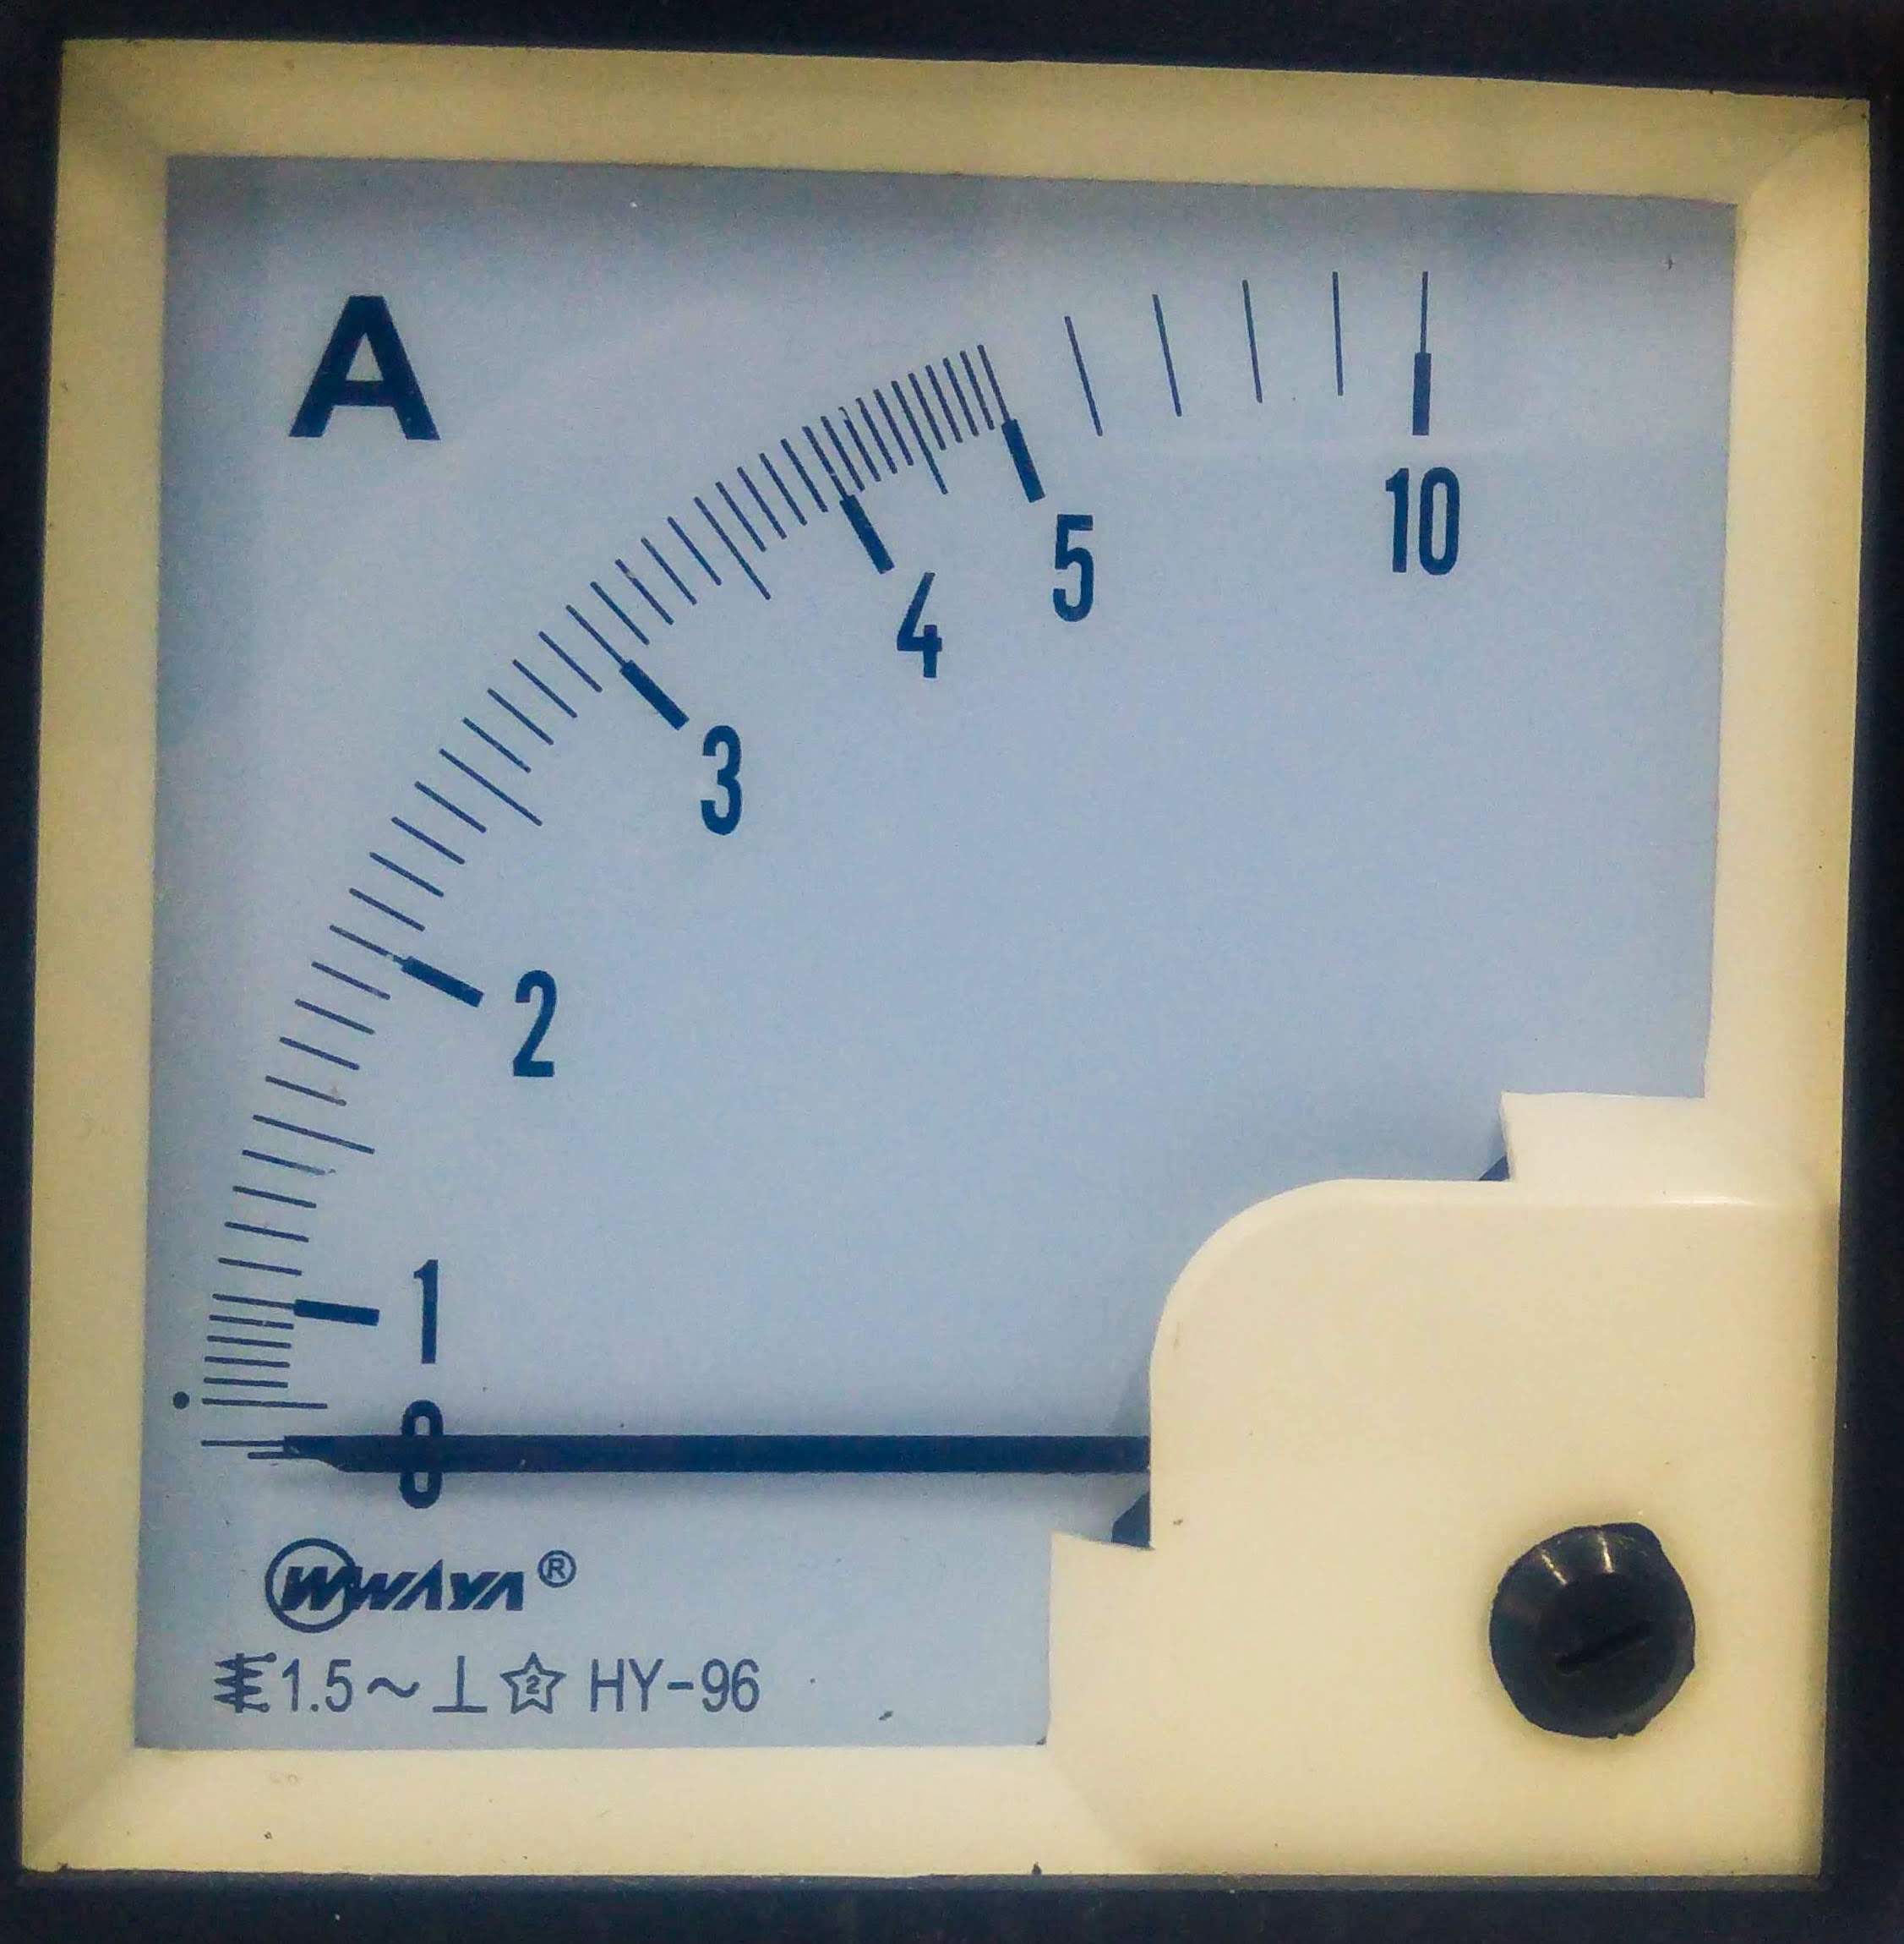
\includegraphics[width=0.5\textwidth]{images/fotos/amperimetro.jpg}
  \caption{Amperímetro}
  \label{fig:amperimetro}
\end{figure}

\subsection{Óhmetro}
\section{Vatímetro}

\begin{figure}[htbp]
  \centering
  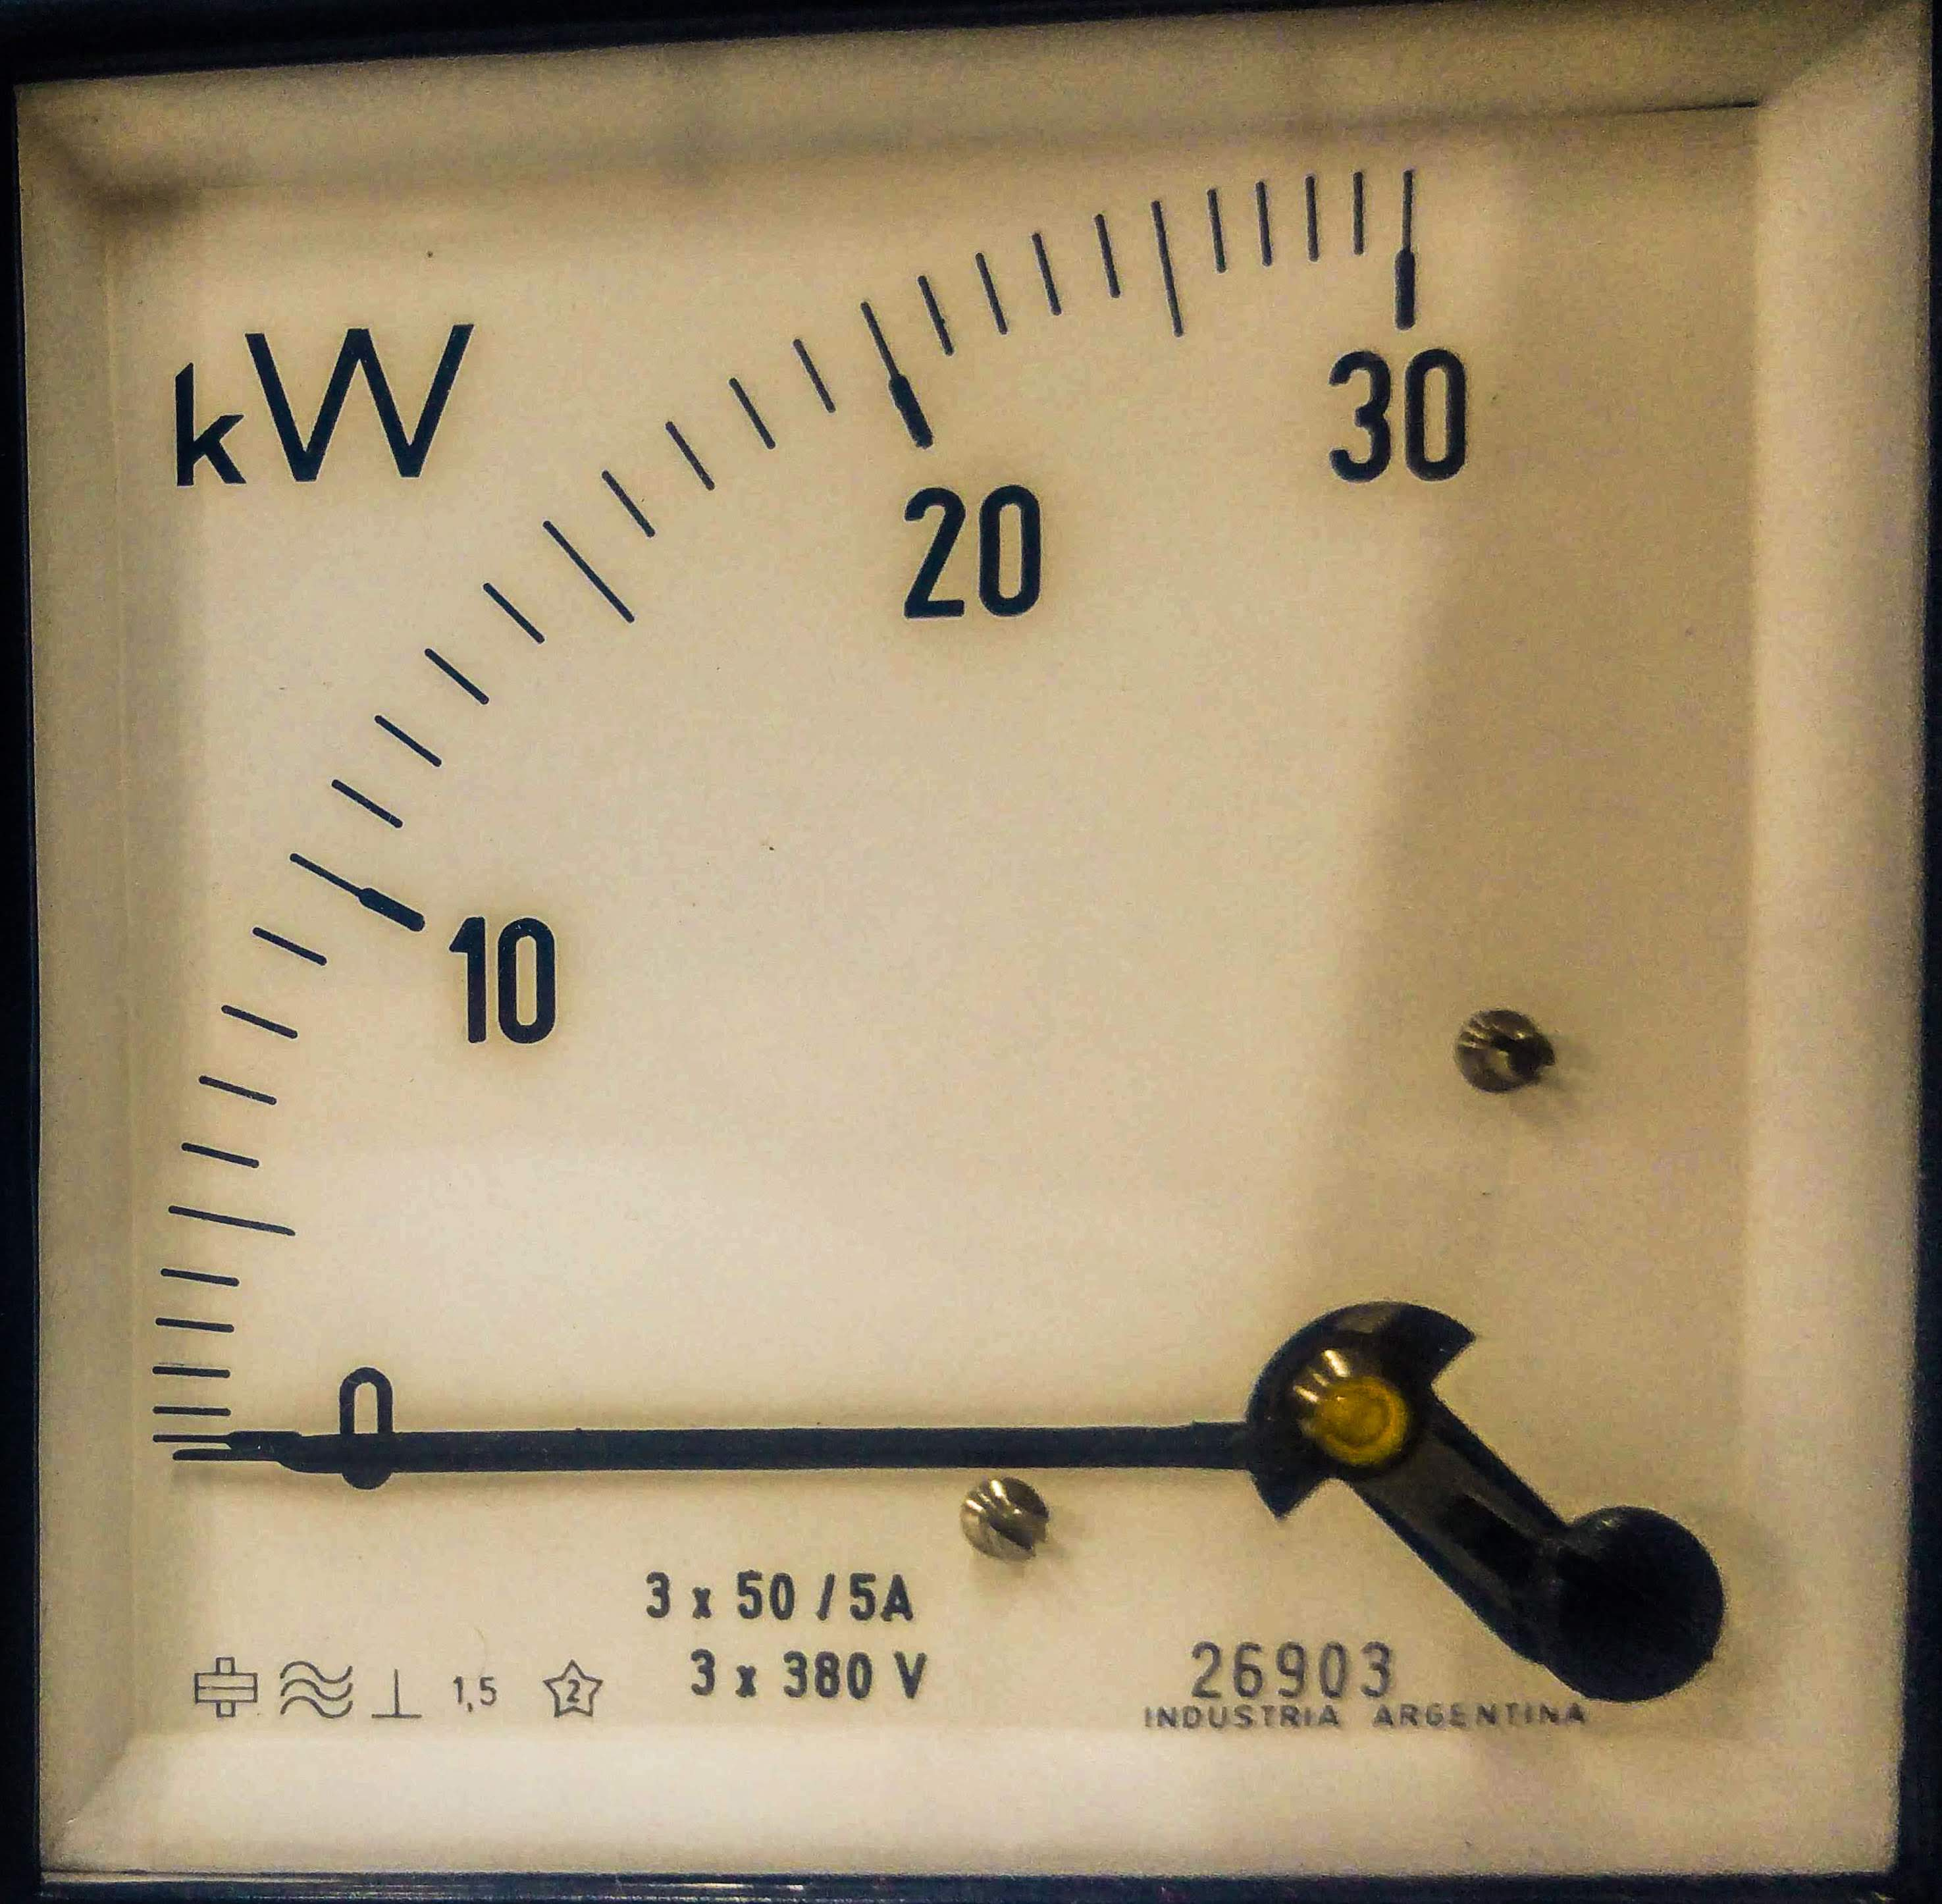
\includegraphics[width=0.5\textwidth,height=\textheight,keepaspectratio]{images/fotos/vatimetro.jpg}
  \caption{Vatímetro analógico}
  \label{fig:vatimetro}
\end{figure}

\section{Capacímetro}
\section{Frecuencímetro}

\begin{figure}[htbp]
  \centering
  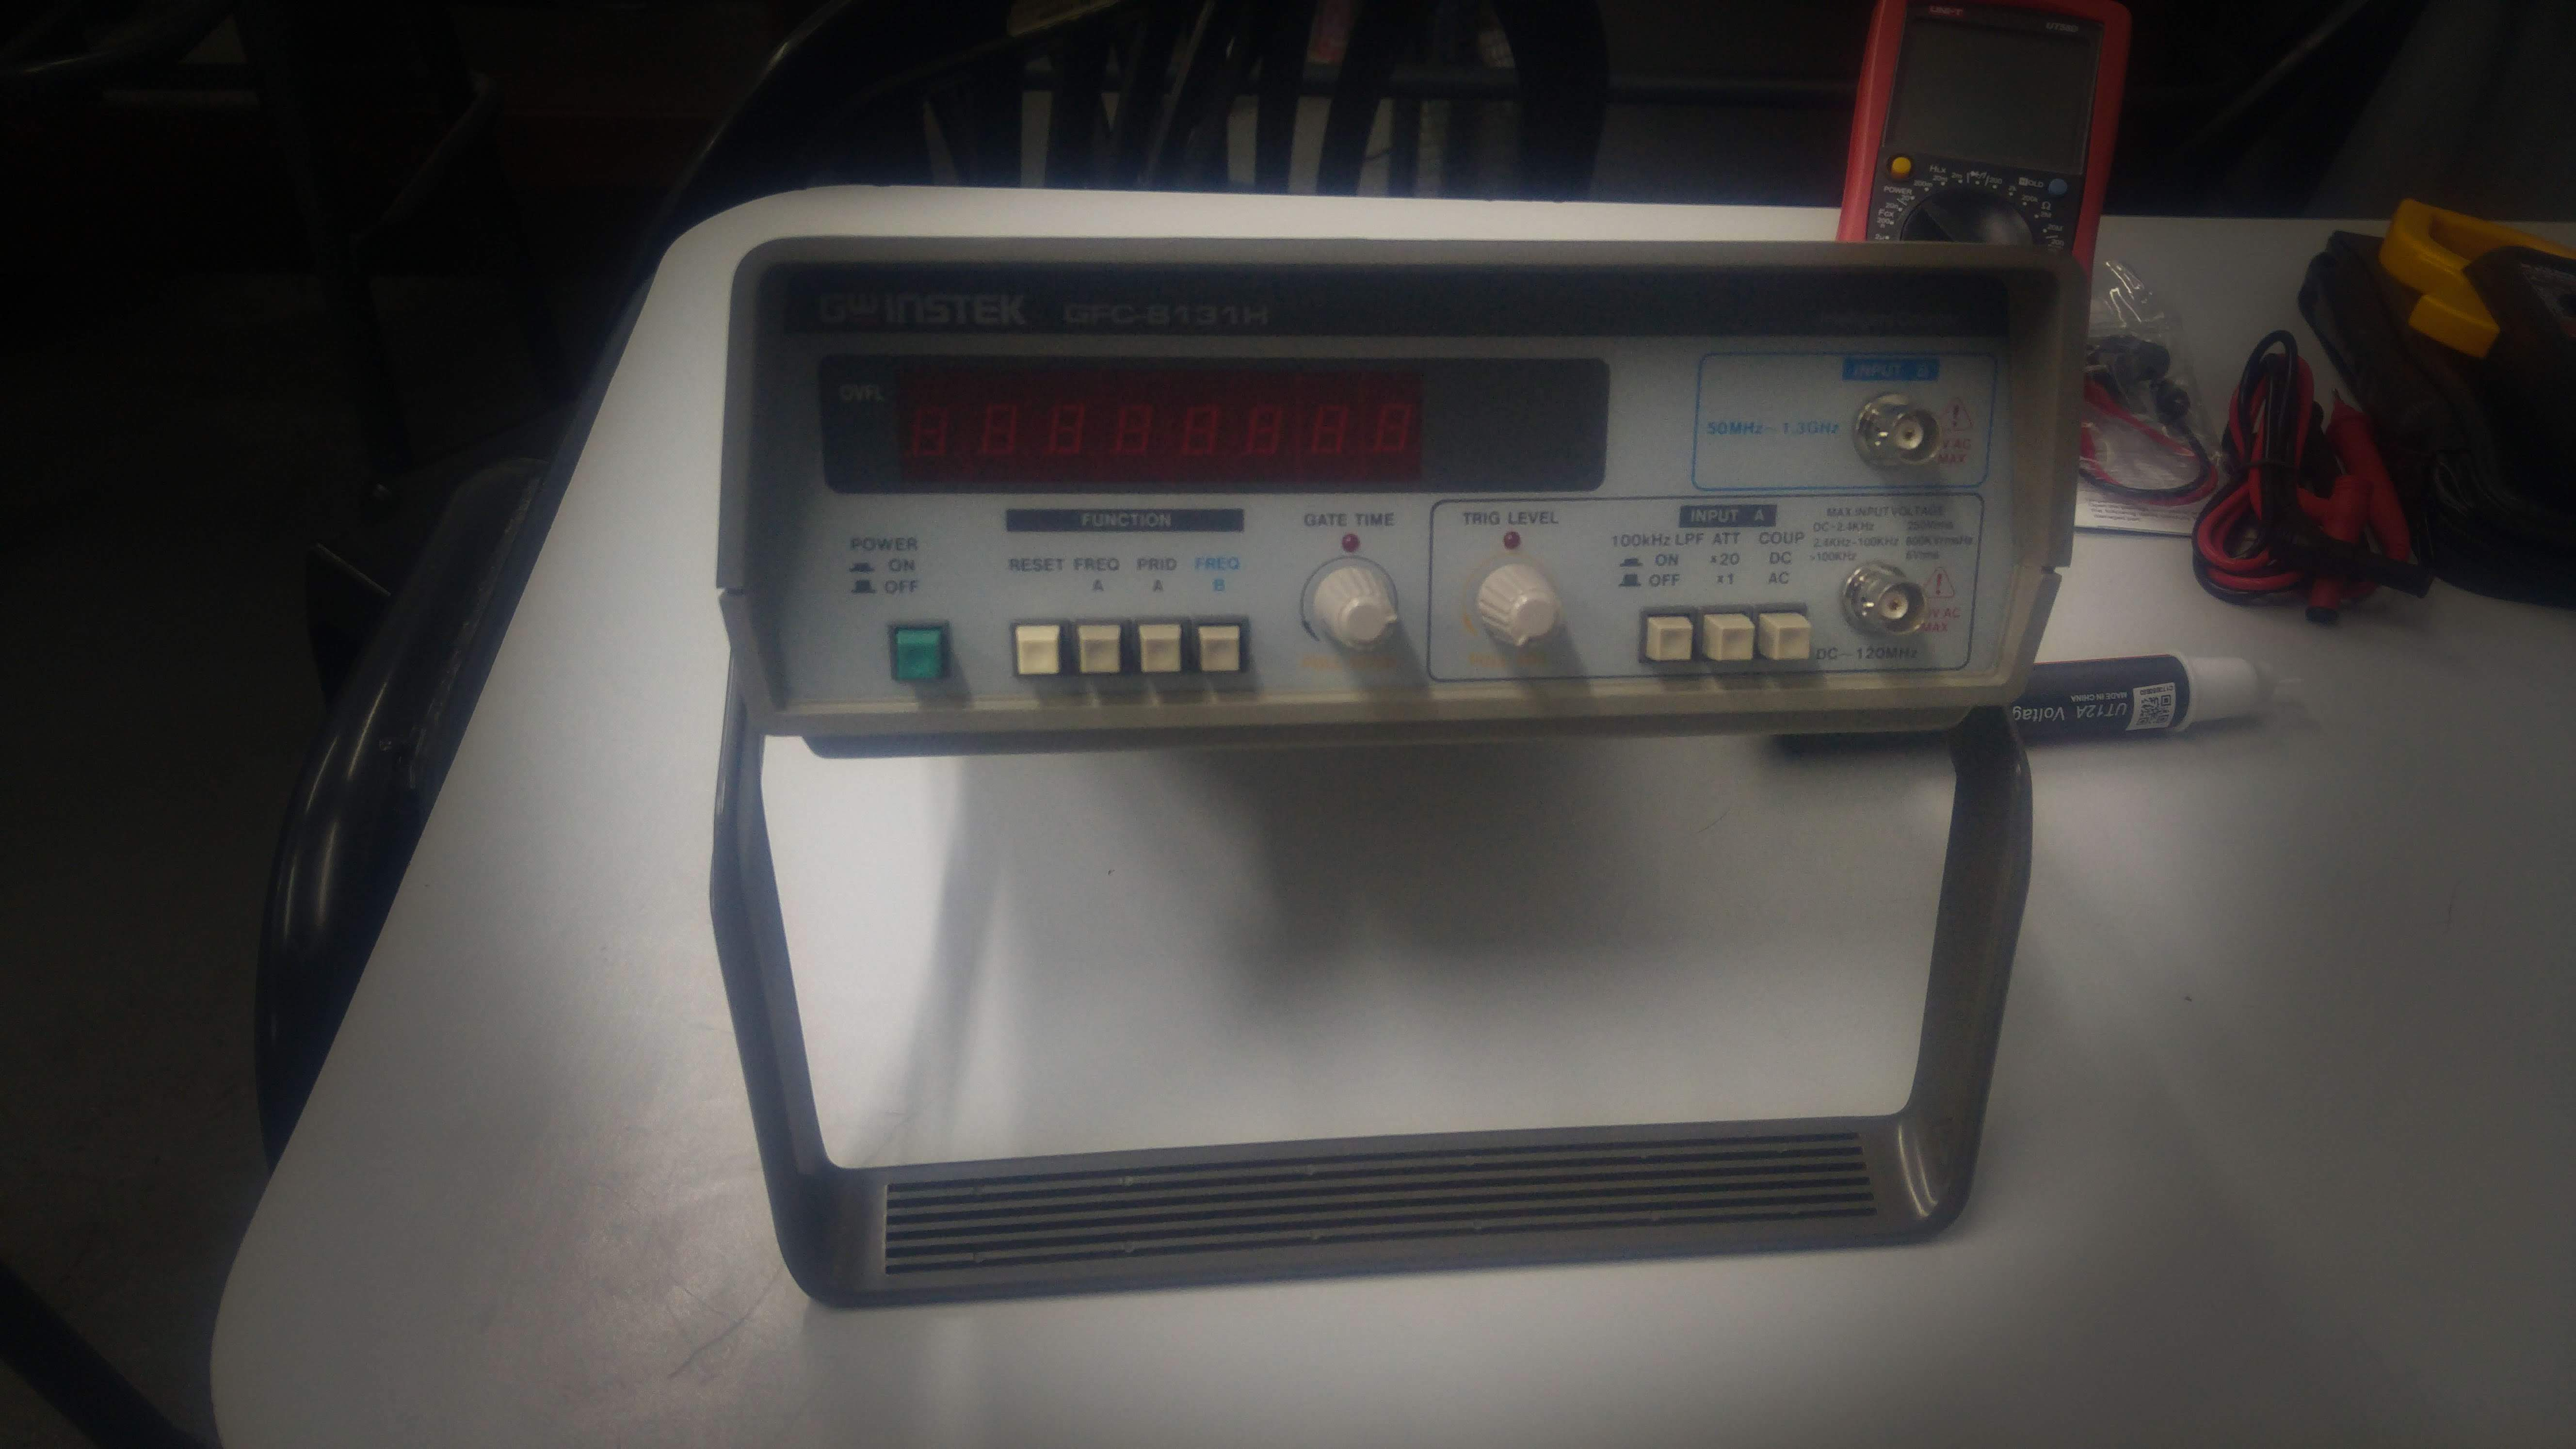
\includegraphics[width=\textwidth,height=\textheight,keepaspectratio]{images/fotos/frecuencimetro.jpg}
  \caption{Frecuencímetro de banco}
  \label{fig:frecuencimetro}
\end{figure}

\section{Pinza amperométrica}

\begin{figure}[htbp]
  \centering
  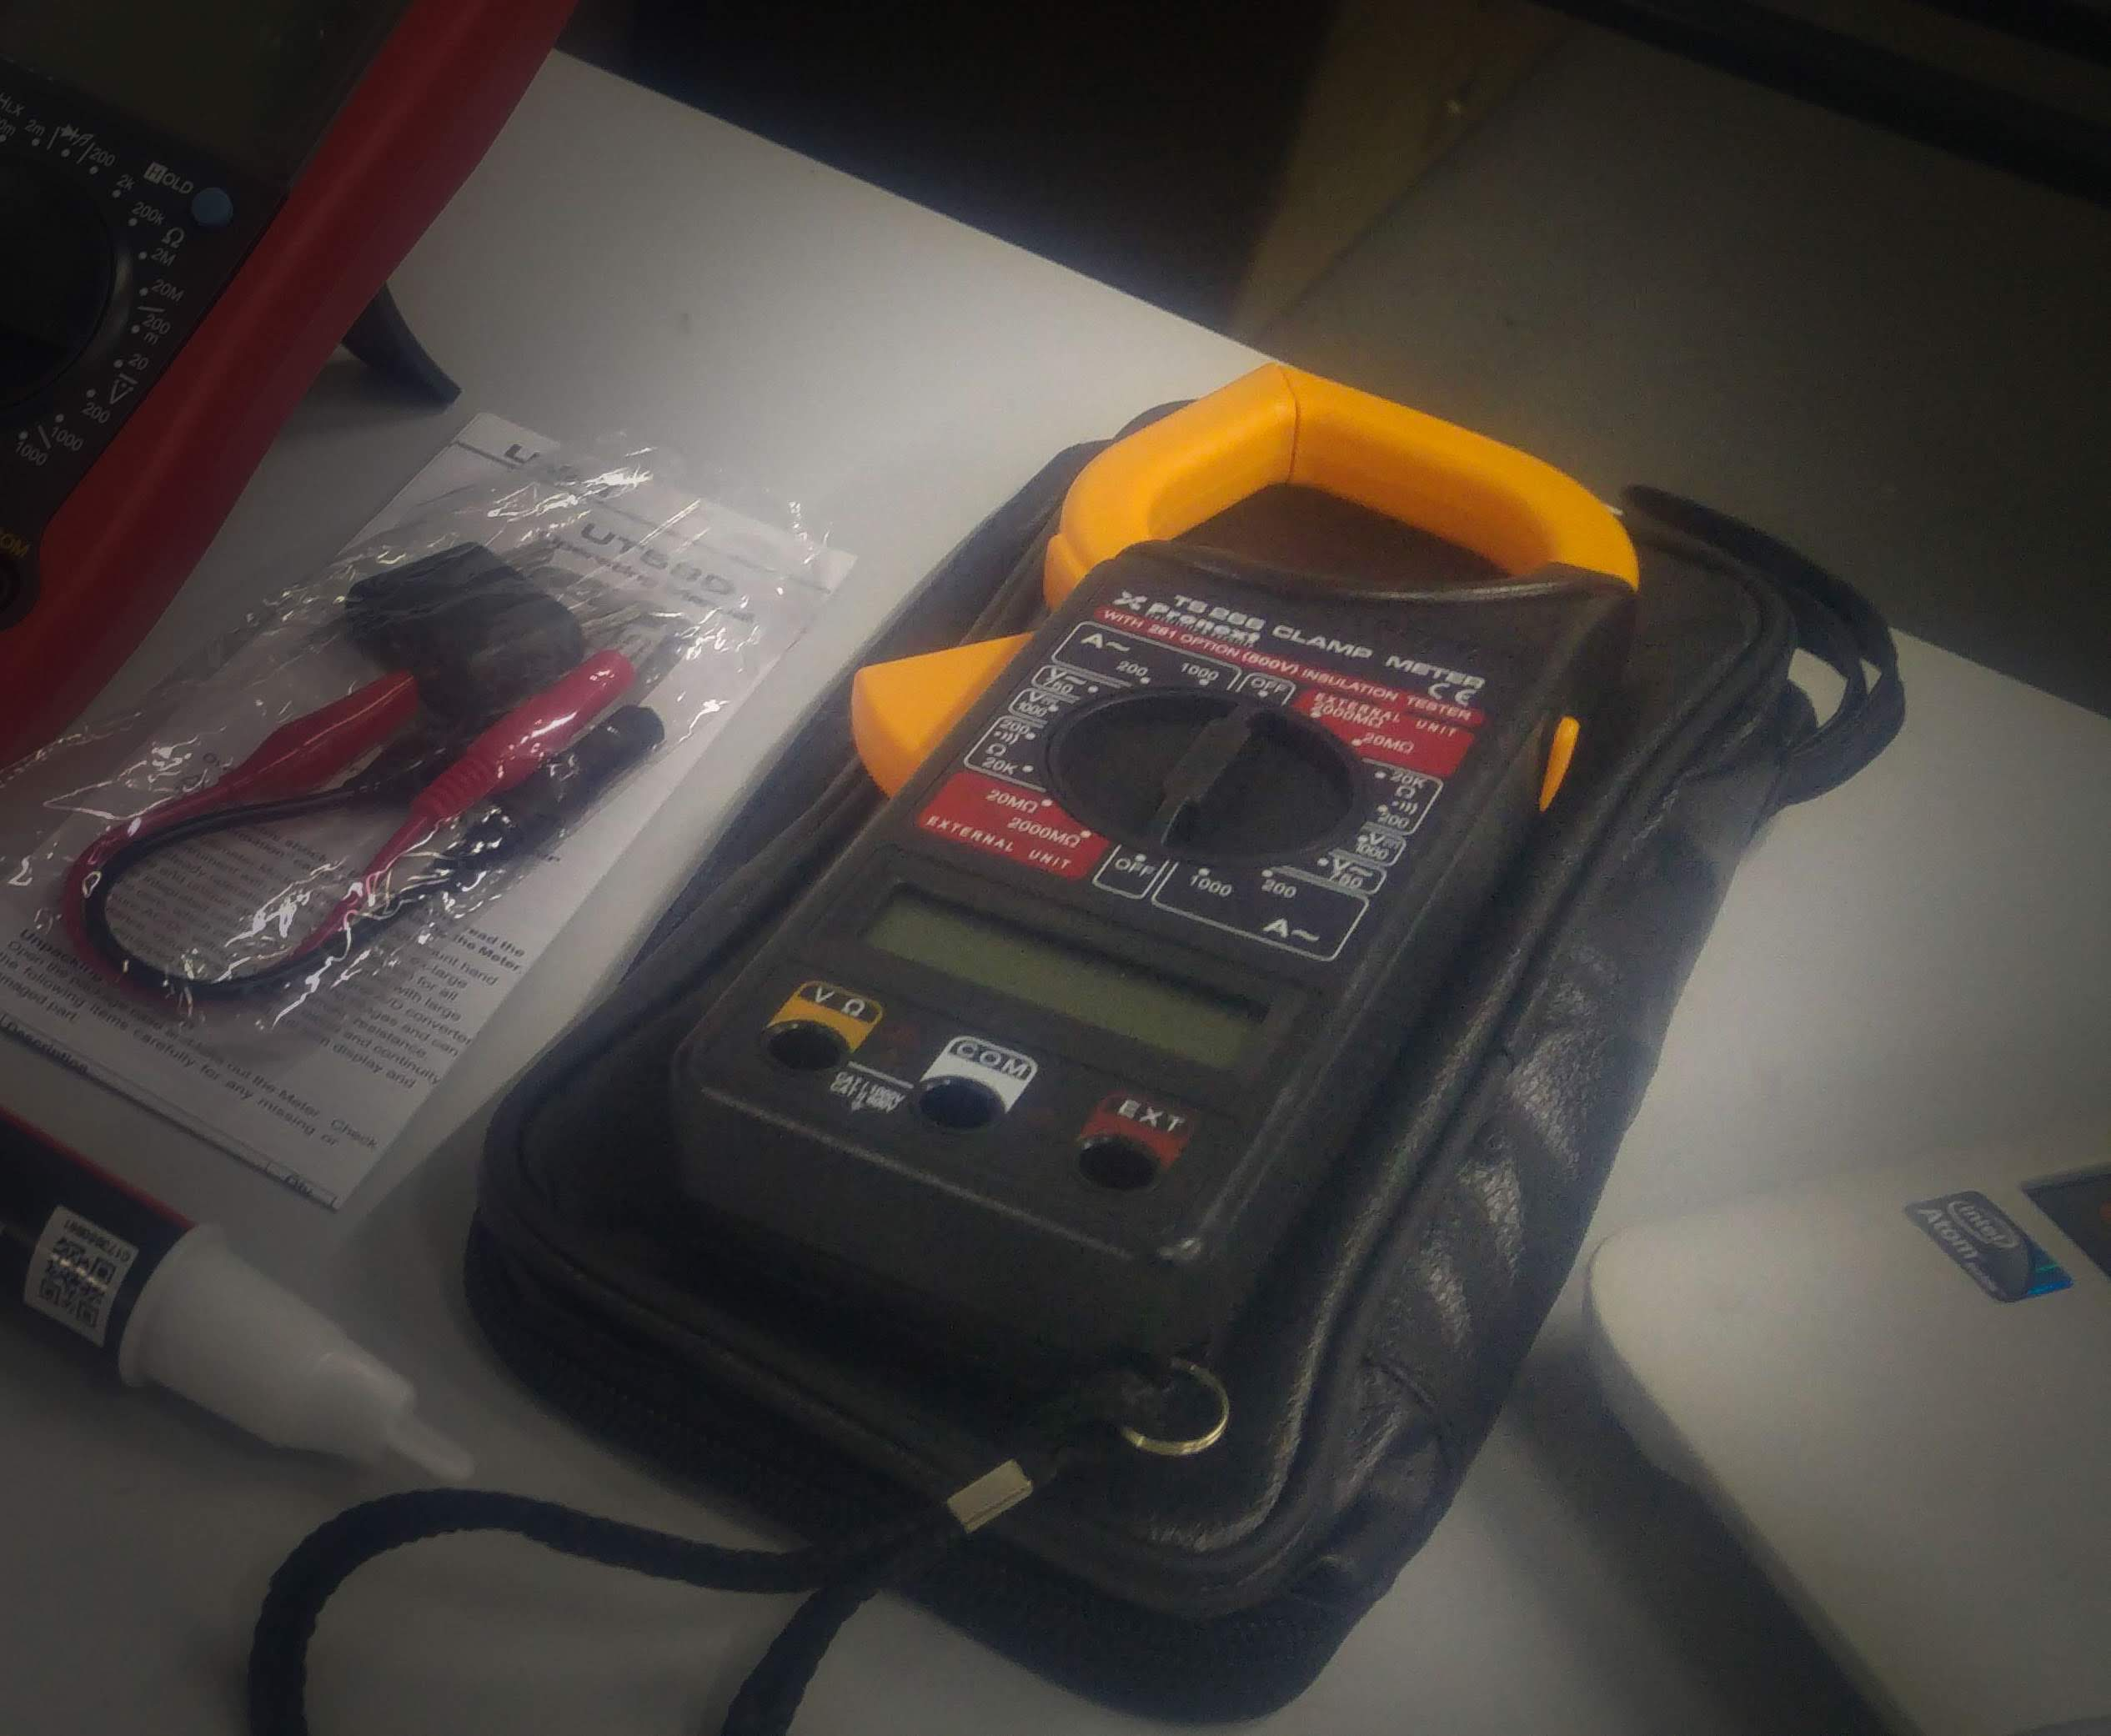
\includegraphics[width=0.3\textwidth,height=\textheight,keepaspectratio]{images/fotos/pinza1.jpg}
  \caption{Pinza amperométrica}
  \label{fig:pinza_amperometrica}
\end{figure}

\begin{figure}[htbp]
  \centering
  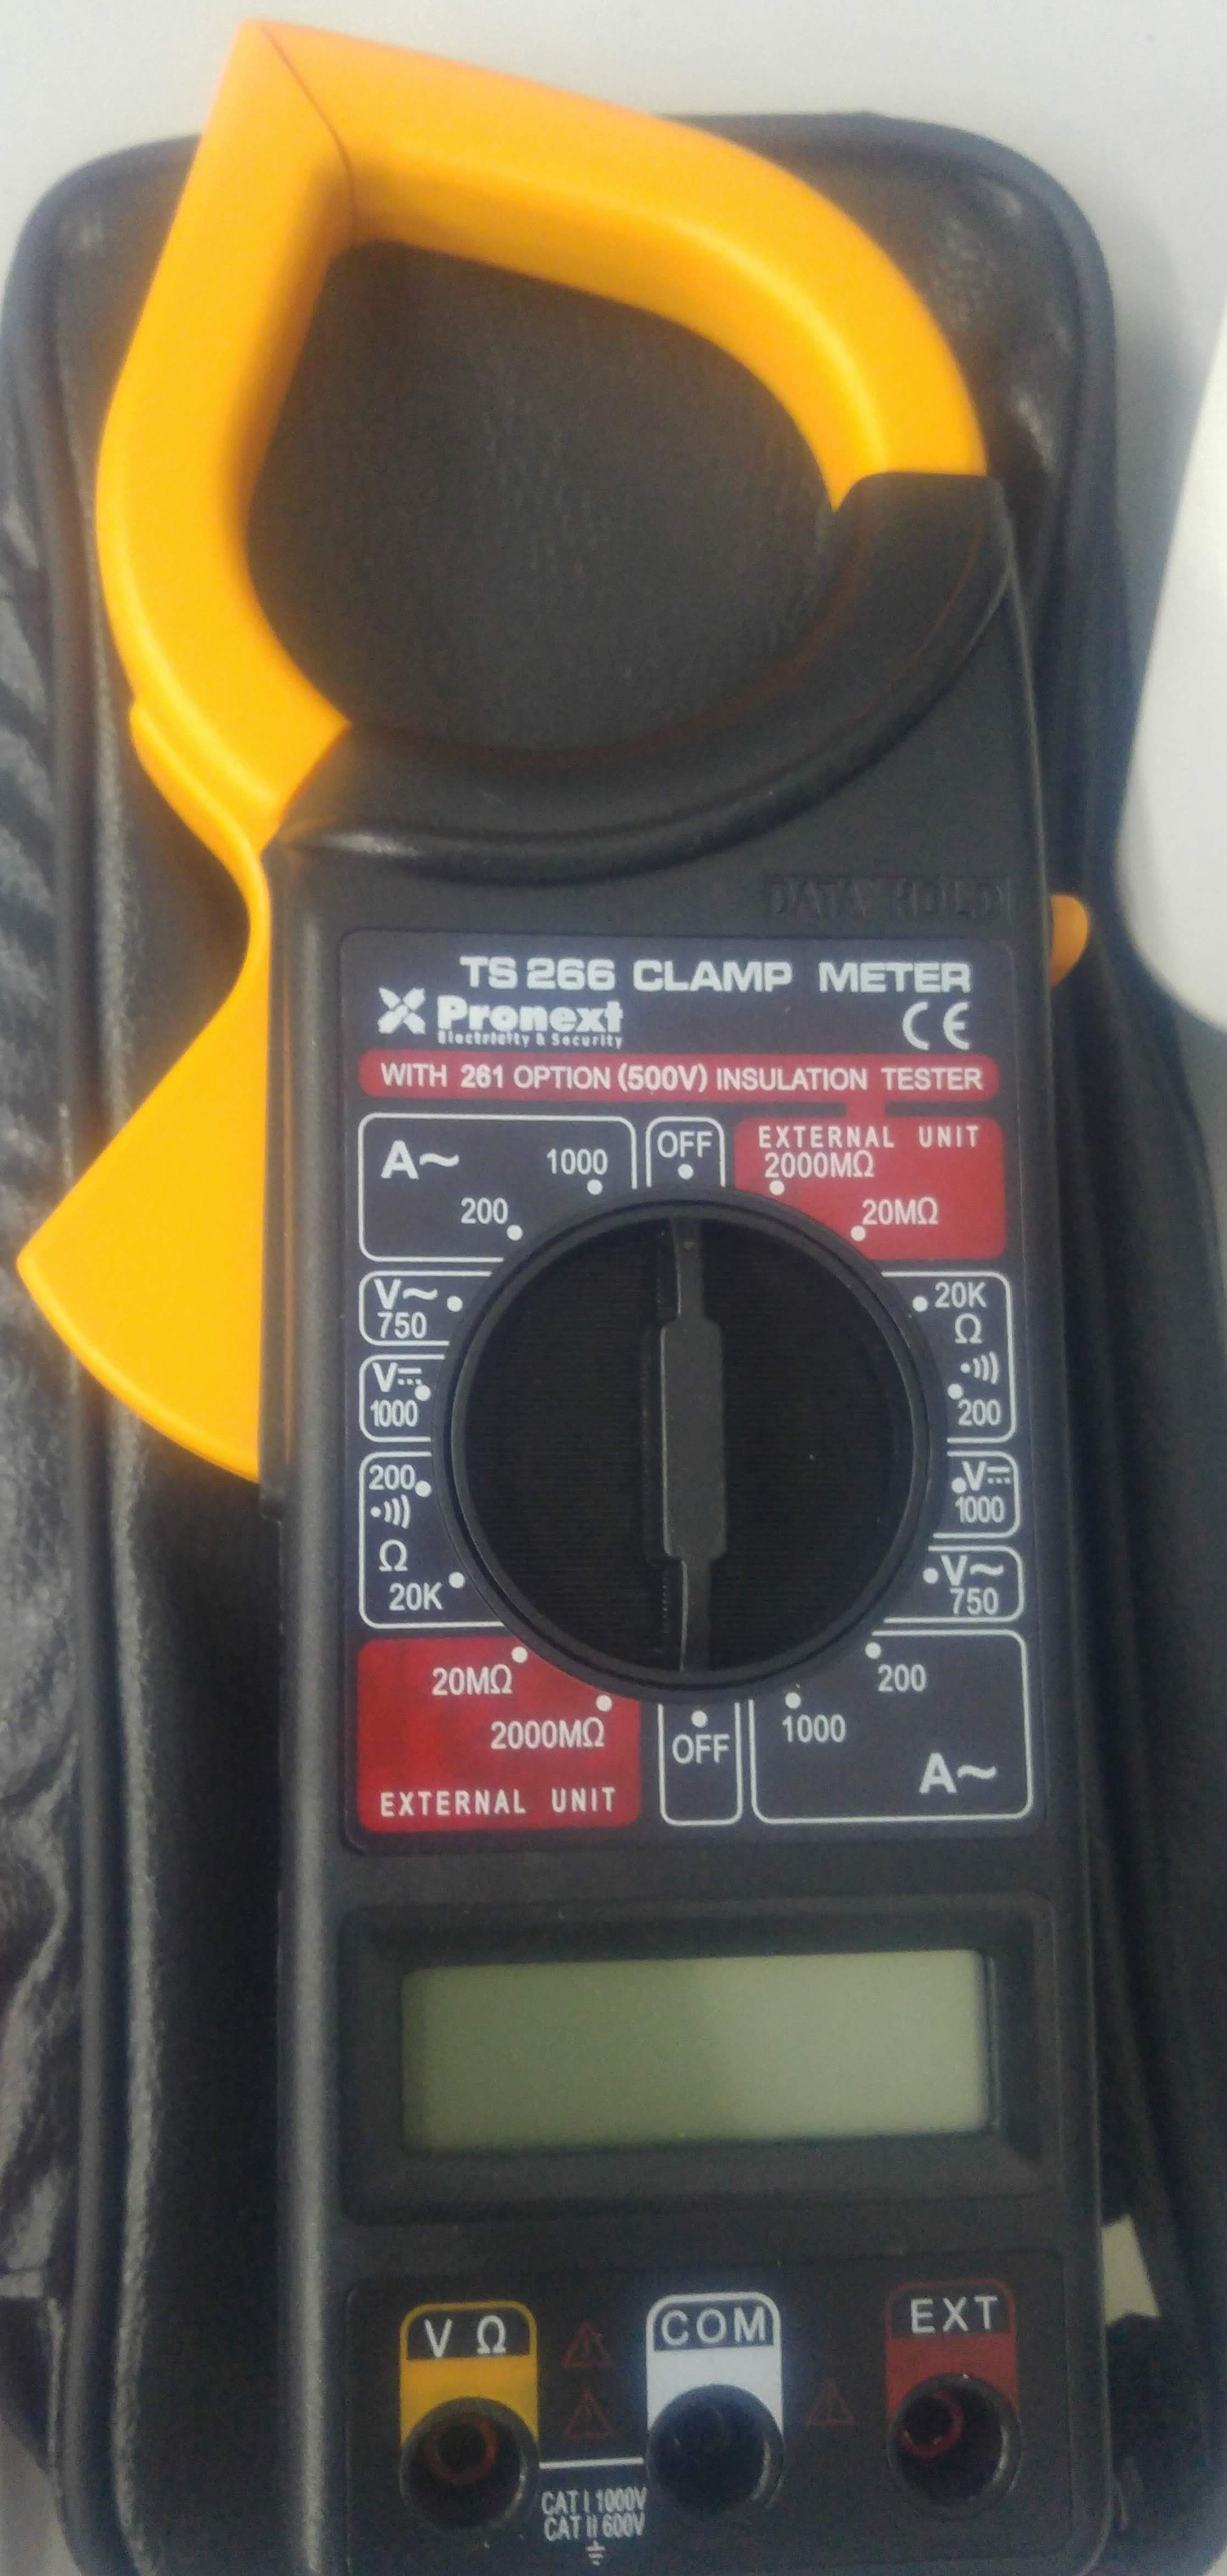
\includegraphics[width=\textwidth,height=\textheight,keepaspectratio]{images/fotos/pinza2.jpg}
  \caption{Vista frontal de pinza amperométrica}
  \label{fig:pinza_amperometrica}
\end{figure}

\section{Megóhmetro, megger o medidor de aislamiento eléctrico}

\begin{figure}[htbp]
  \centering
  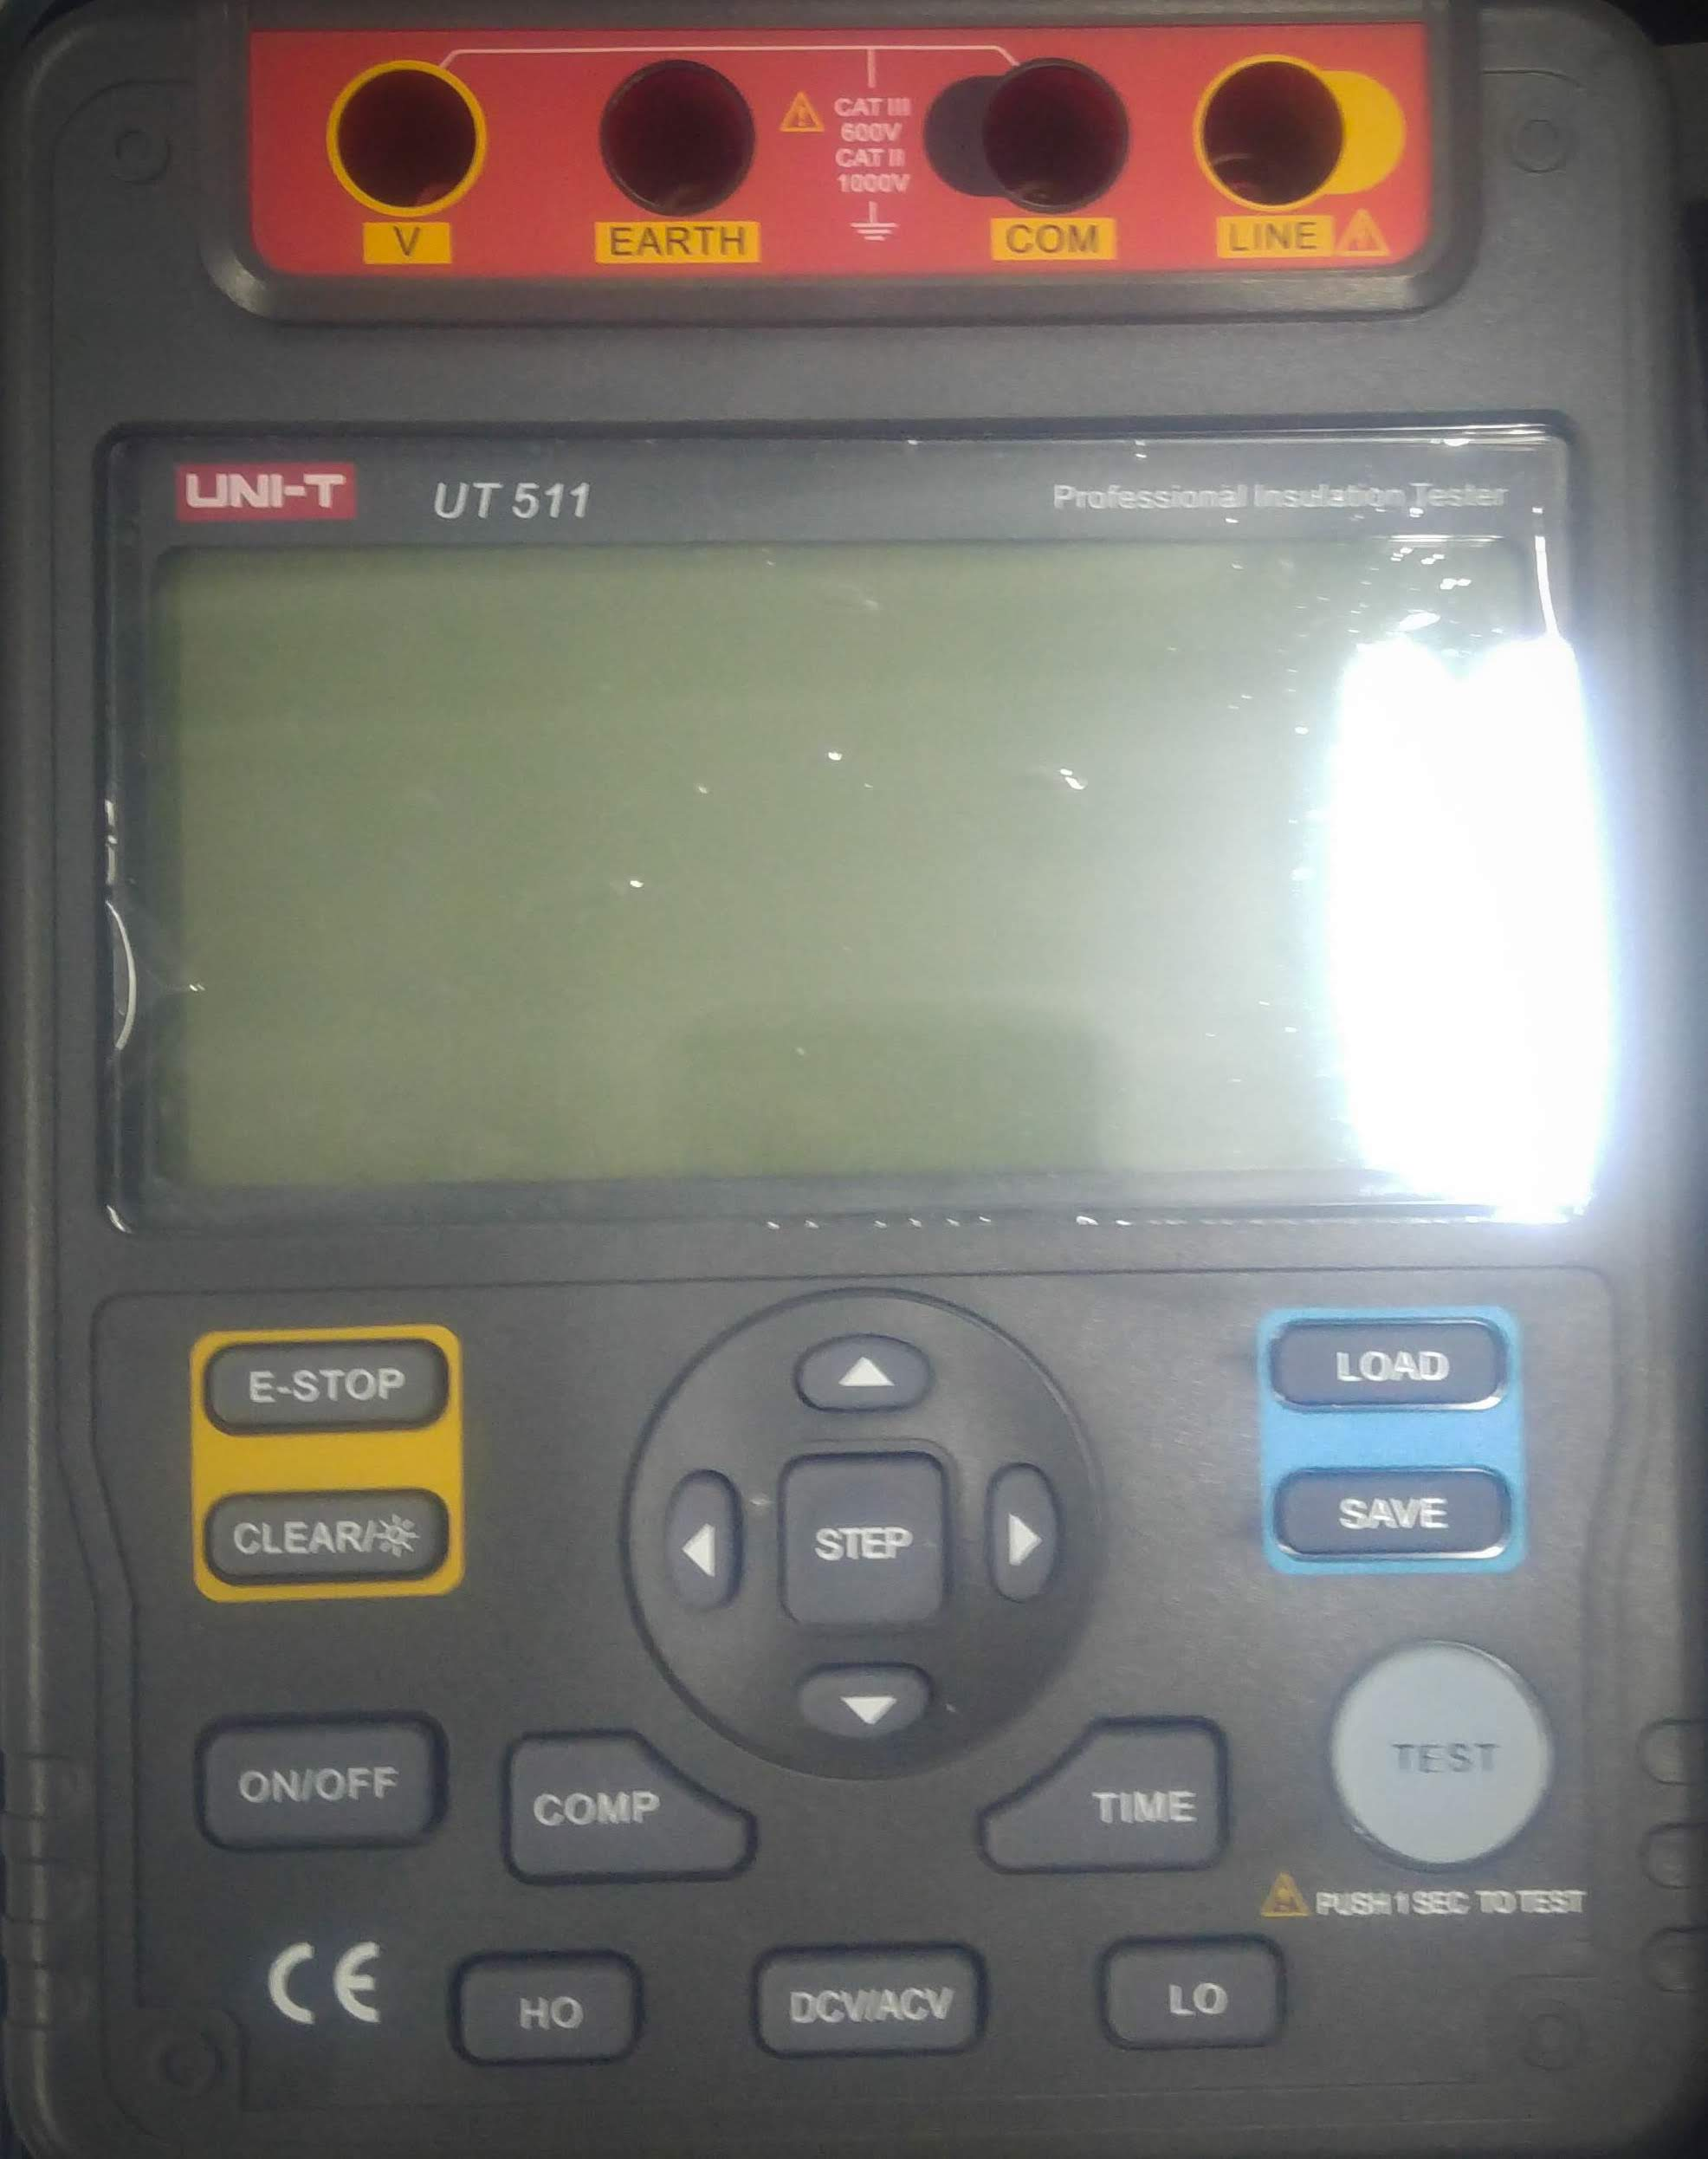
\includegraphics[width=0.5\textwidth,height=\textheight,keepaspectratio]{images/fotos/megger.jpg}
  \caption{Vista frontal de medidor de aislamiento}
  \label{fig:medidor_aislamiento}
\end{figure}

\section{Telurímetro o medidor de puesta a tierra}

\begin{figure}[htbp]
  \centering
  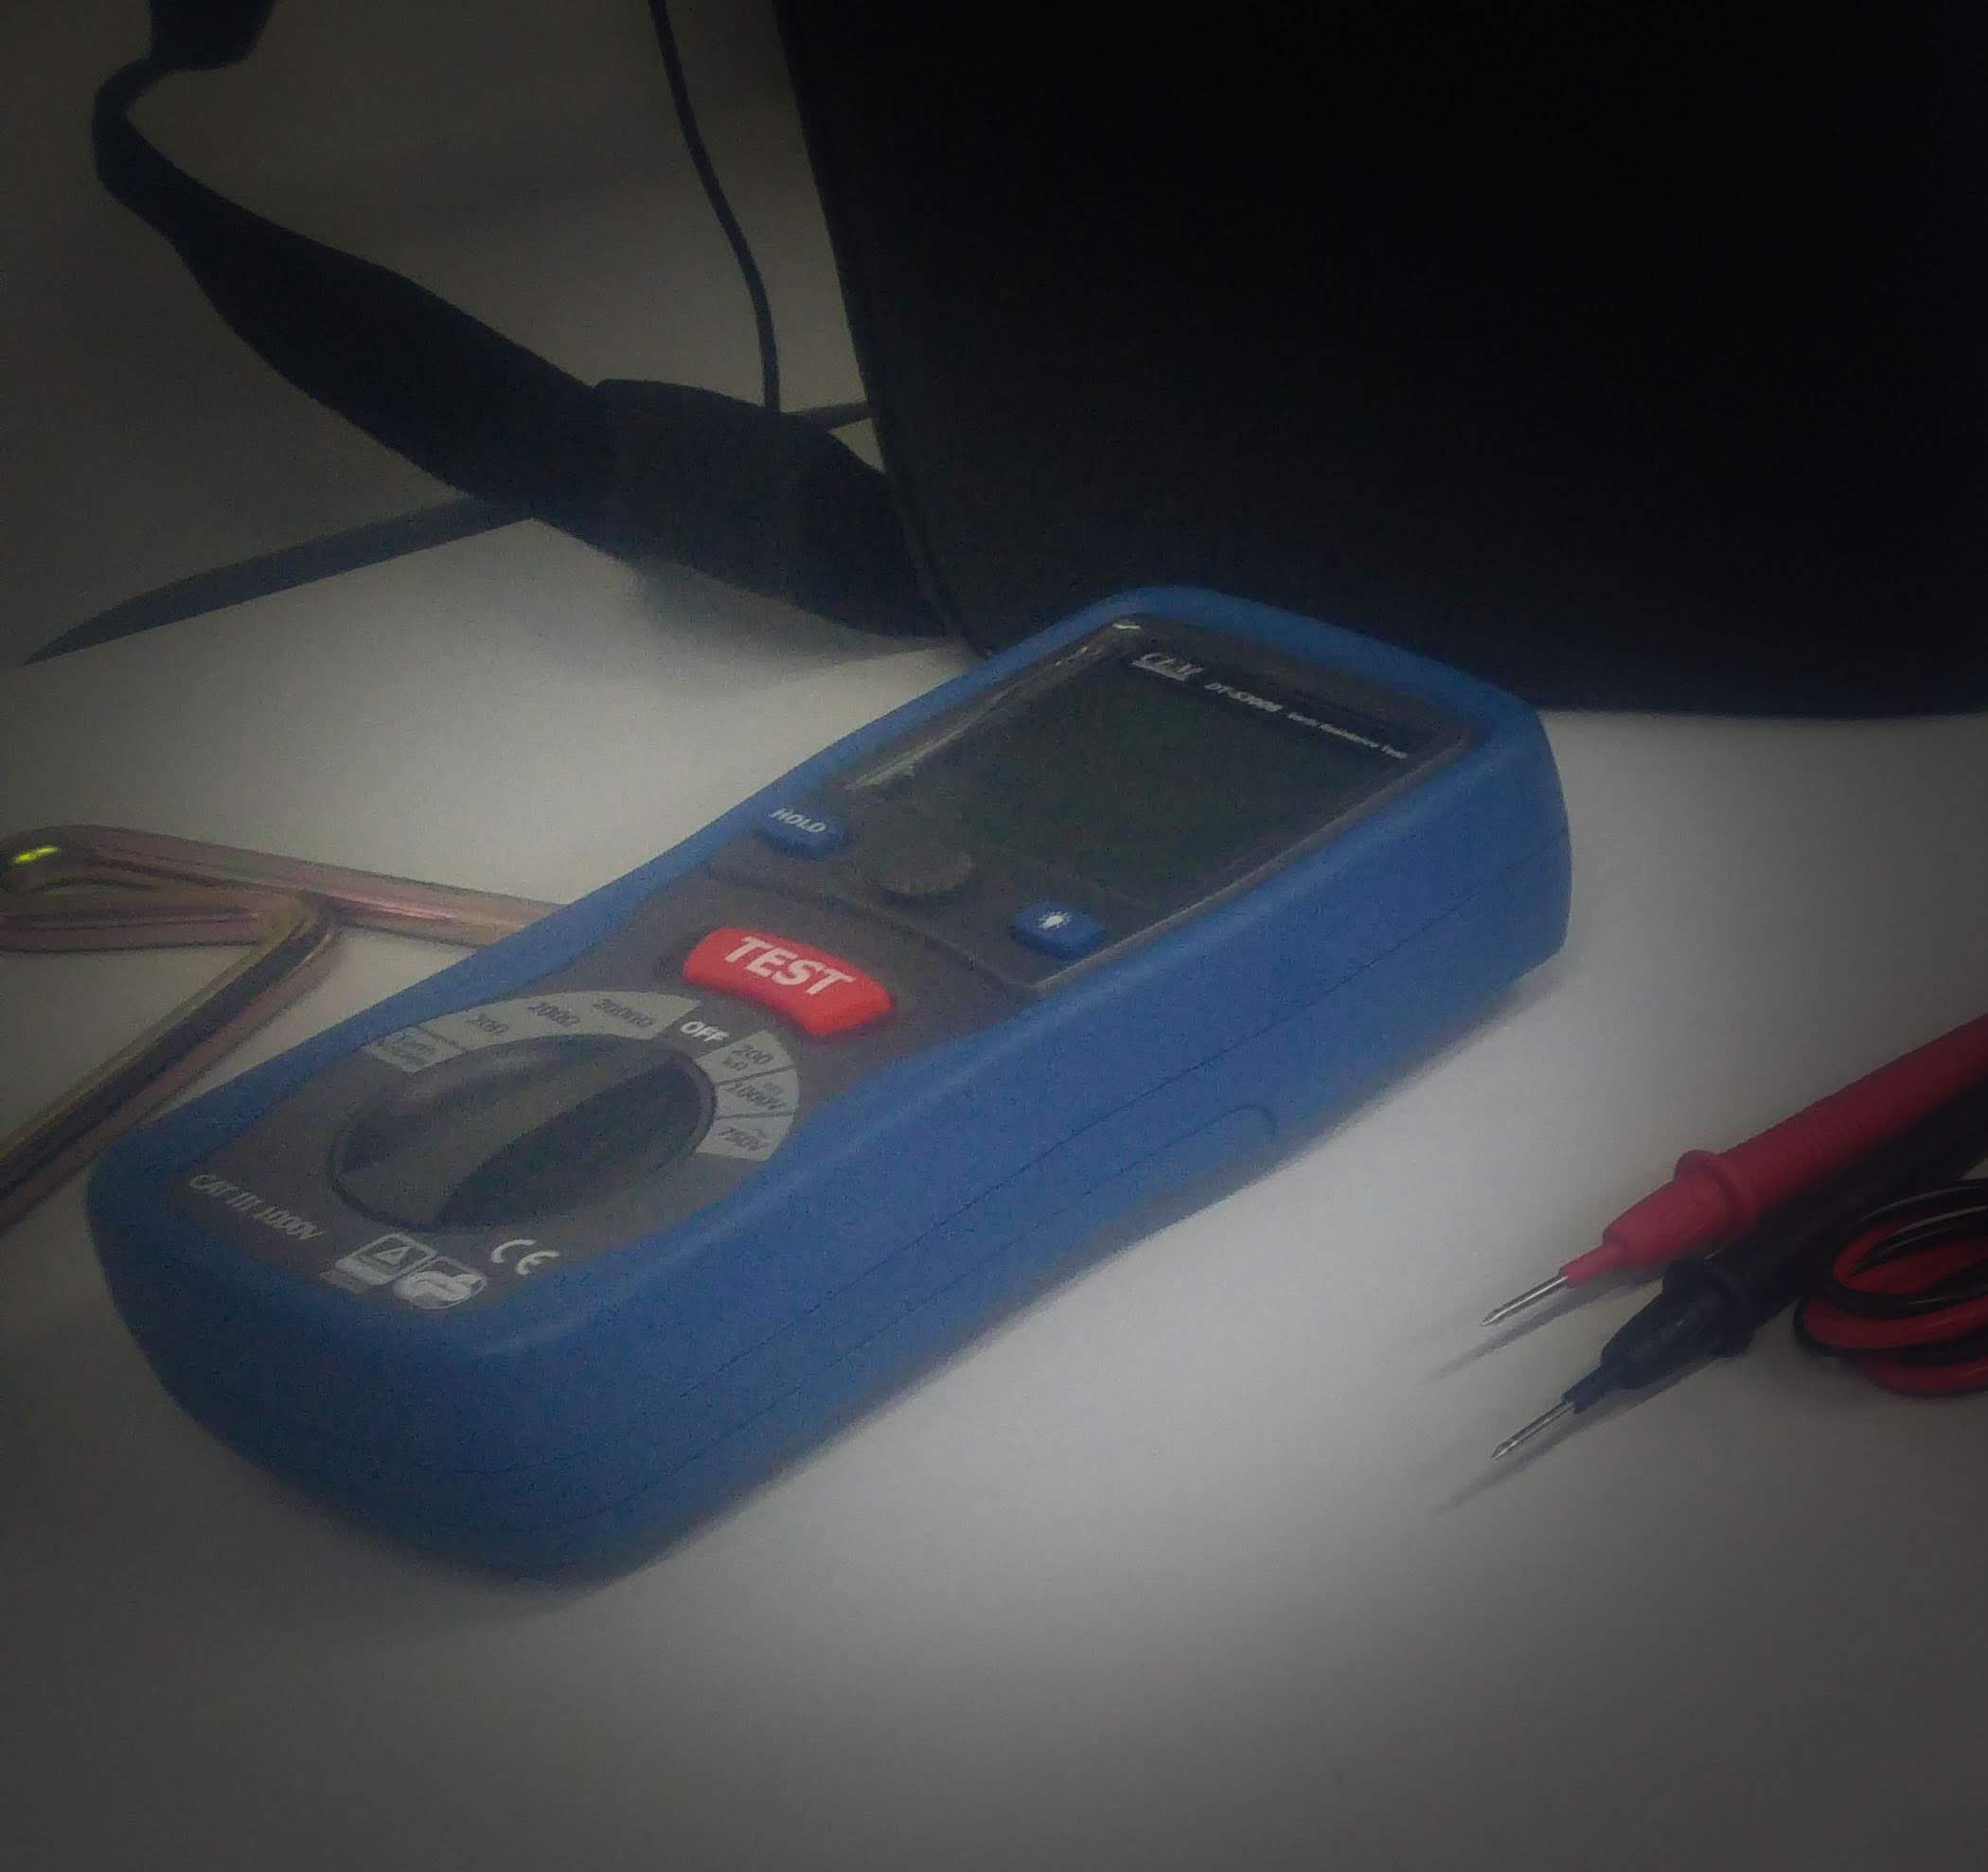
\includegraphics[width=0.5\textwidth,height=\textheight,keepaspectratio]{images/fotos/telurimetro1.jpg}
  \caption{Telurímetro}
  \label{fig:telurimetro}
\end{figure}

\section{Osciloscopio}

\begin{figure}[htbp]
  \centering
  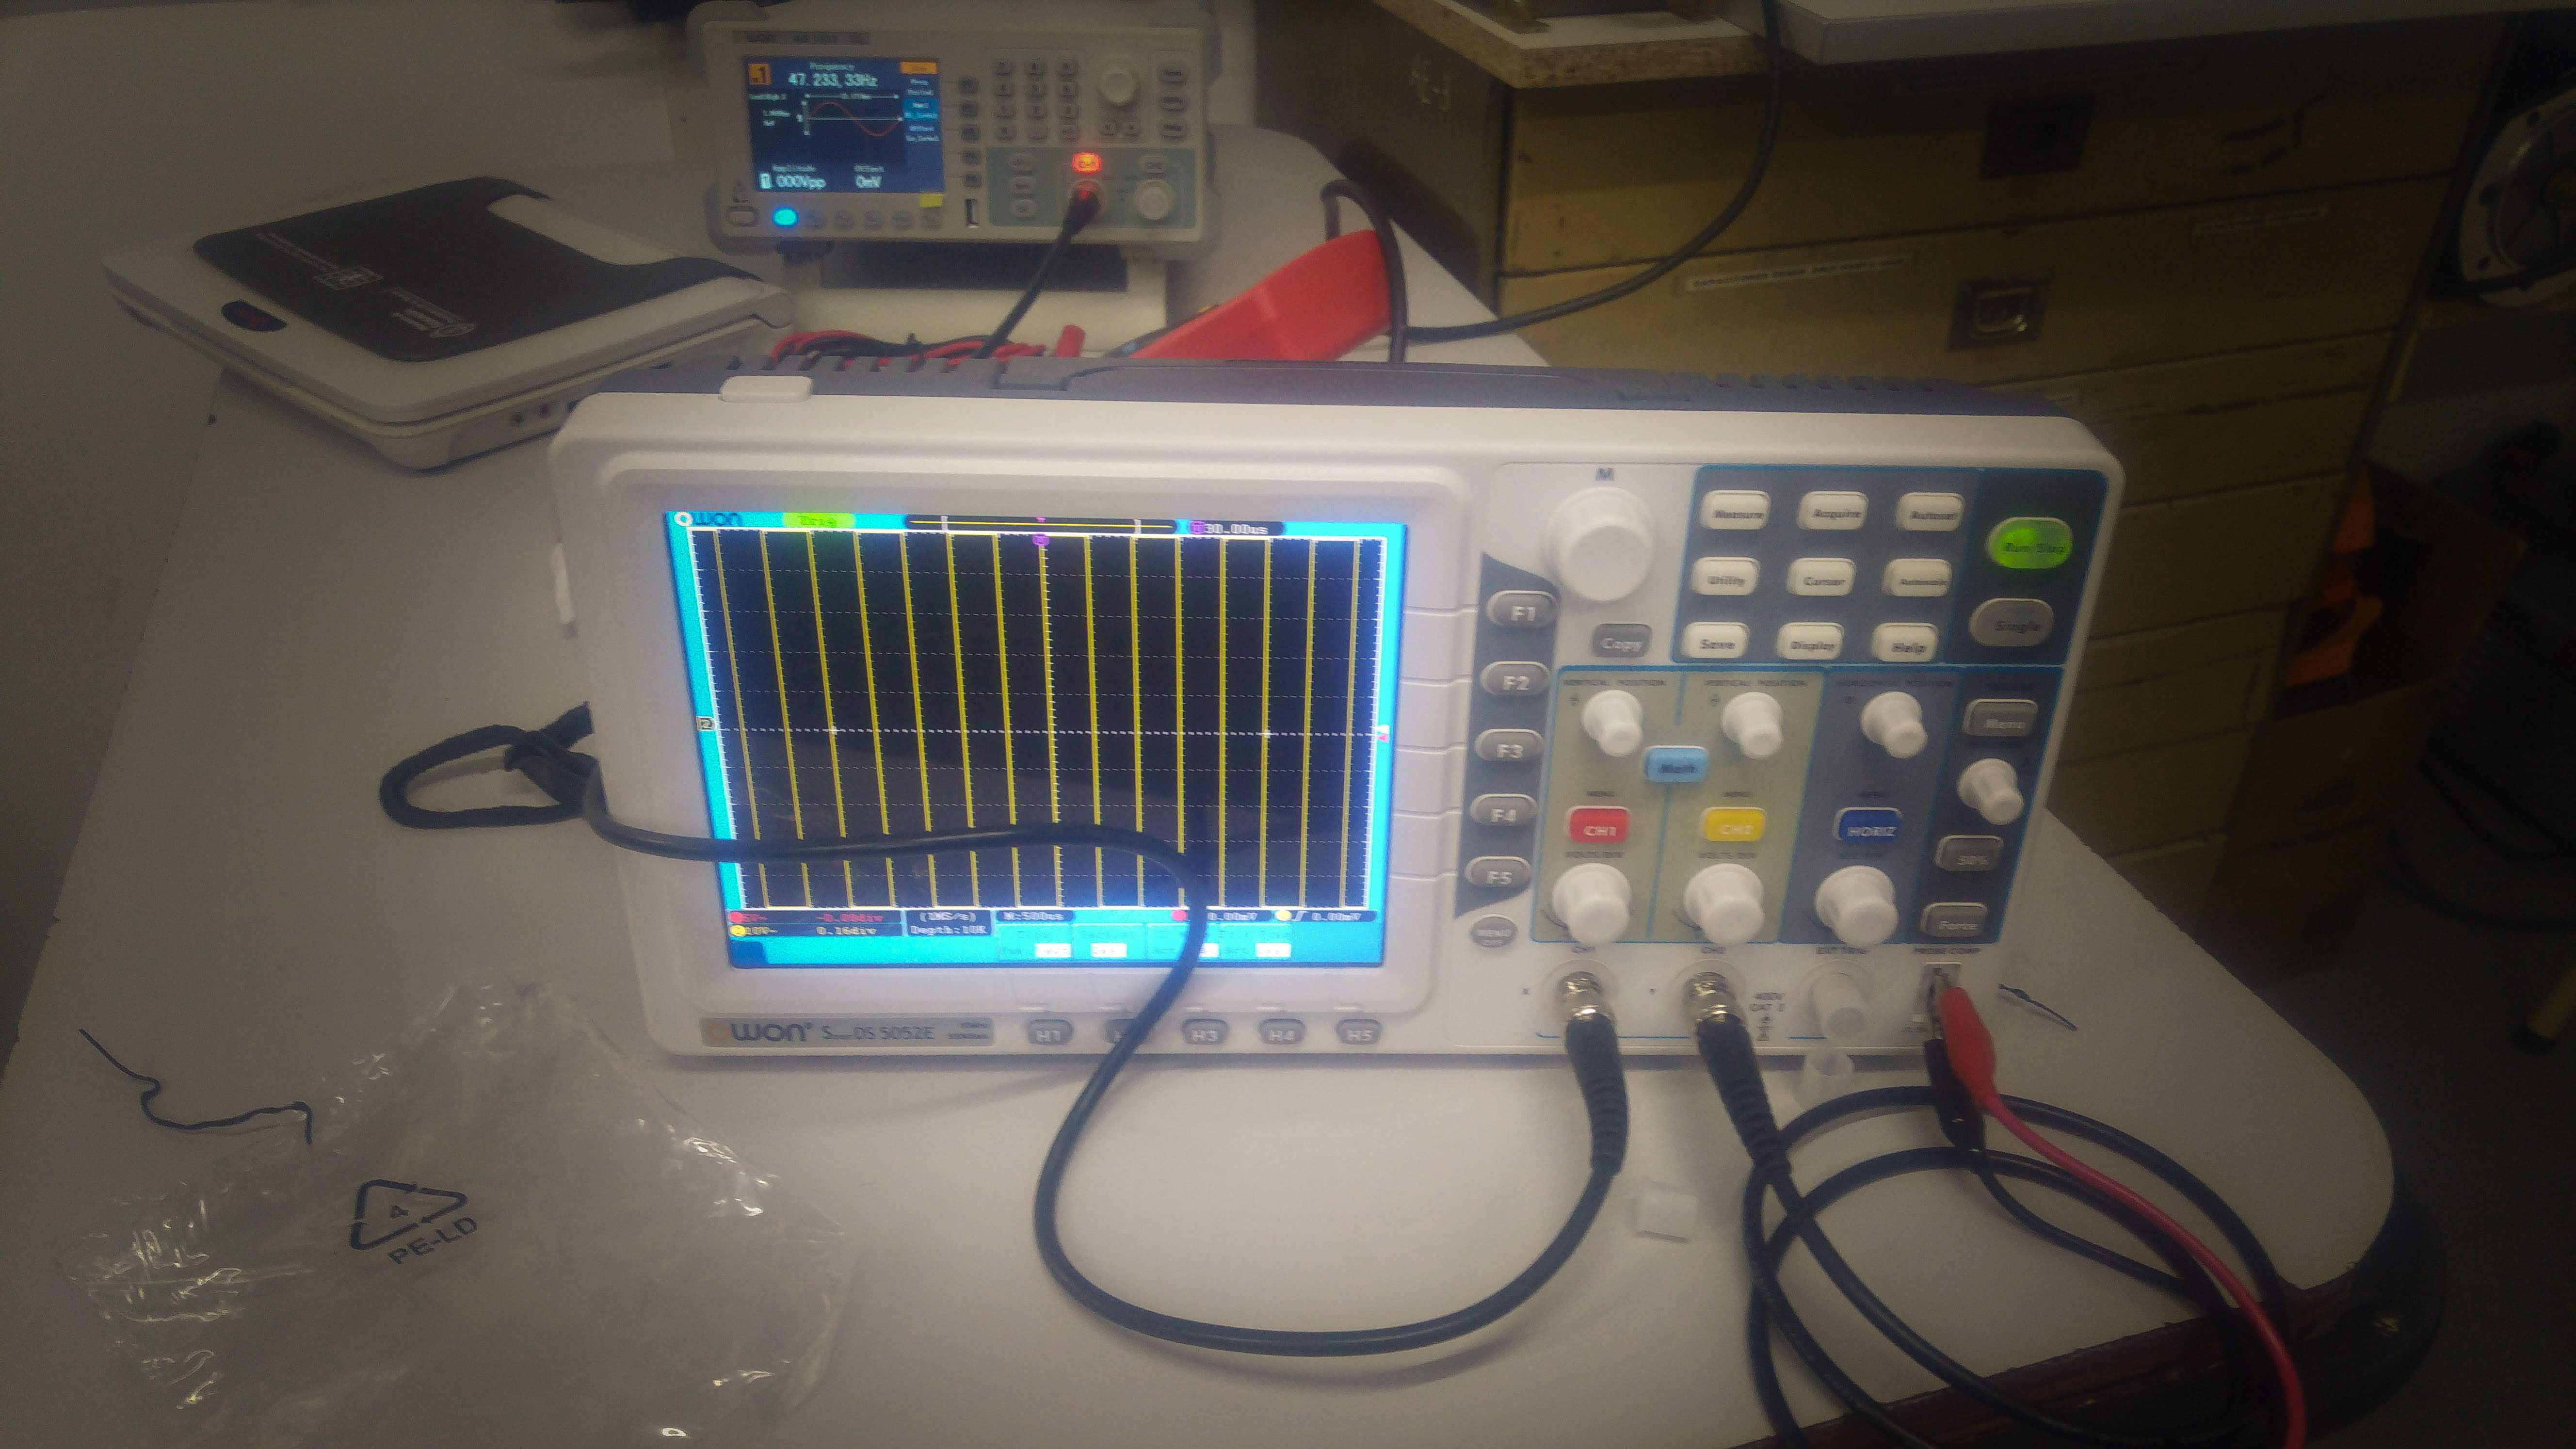
\includegraphics[width=\textwidth,height=\textheight,keepaspectratio]{images/fotos/osciloscopio1.jpg}
  \caption{Osciloscopio con pantalla LED}
  \label{fig:osciloscopio_led}
\end{figure}

\begin{figure}[htbp]
  \centering
  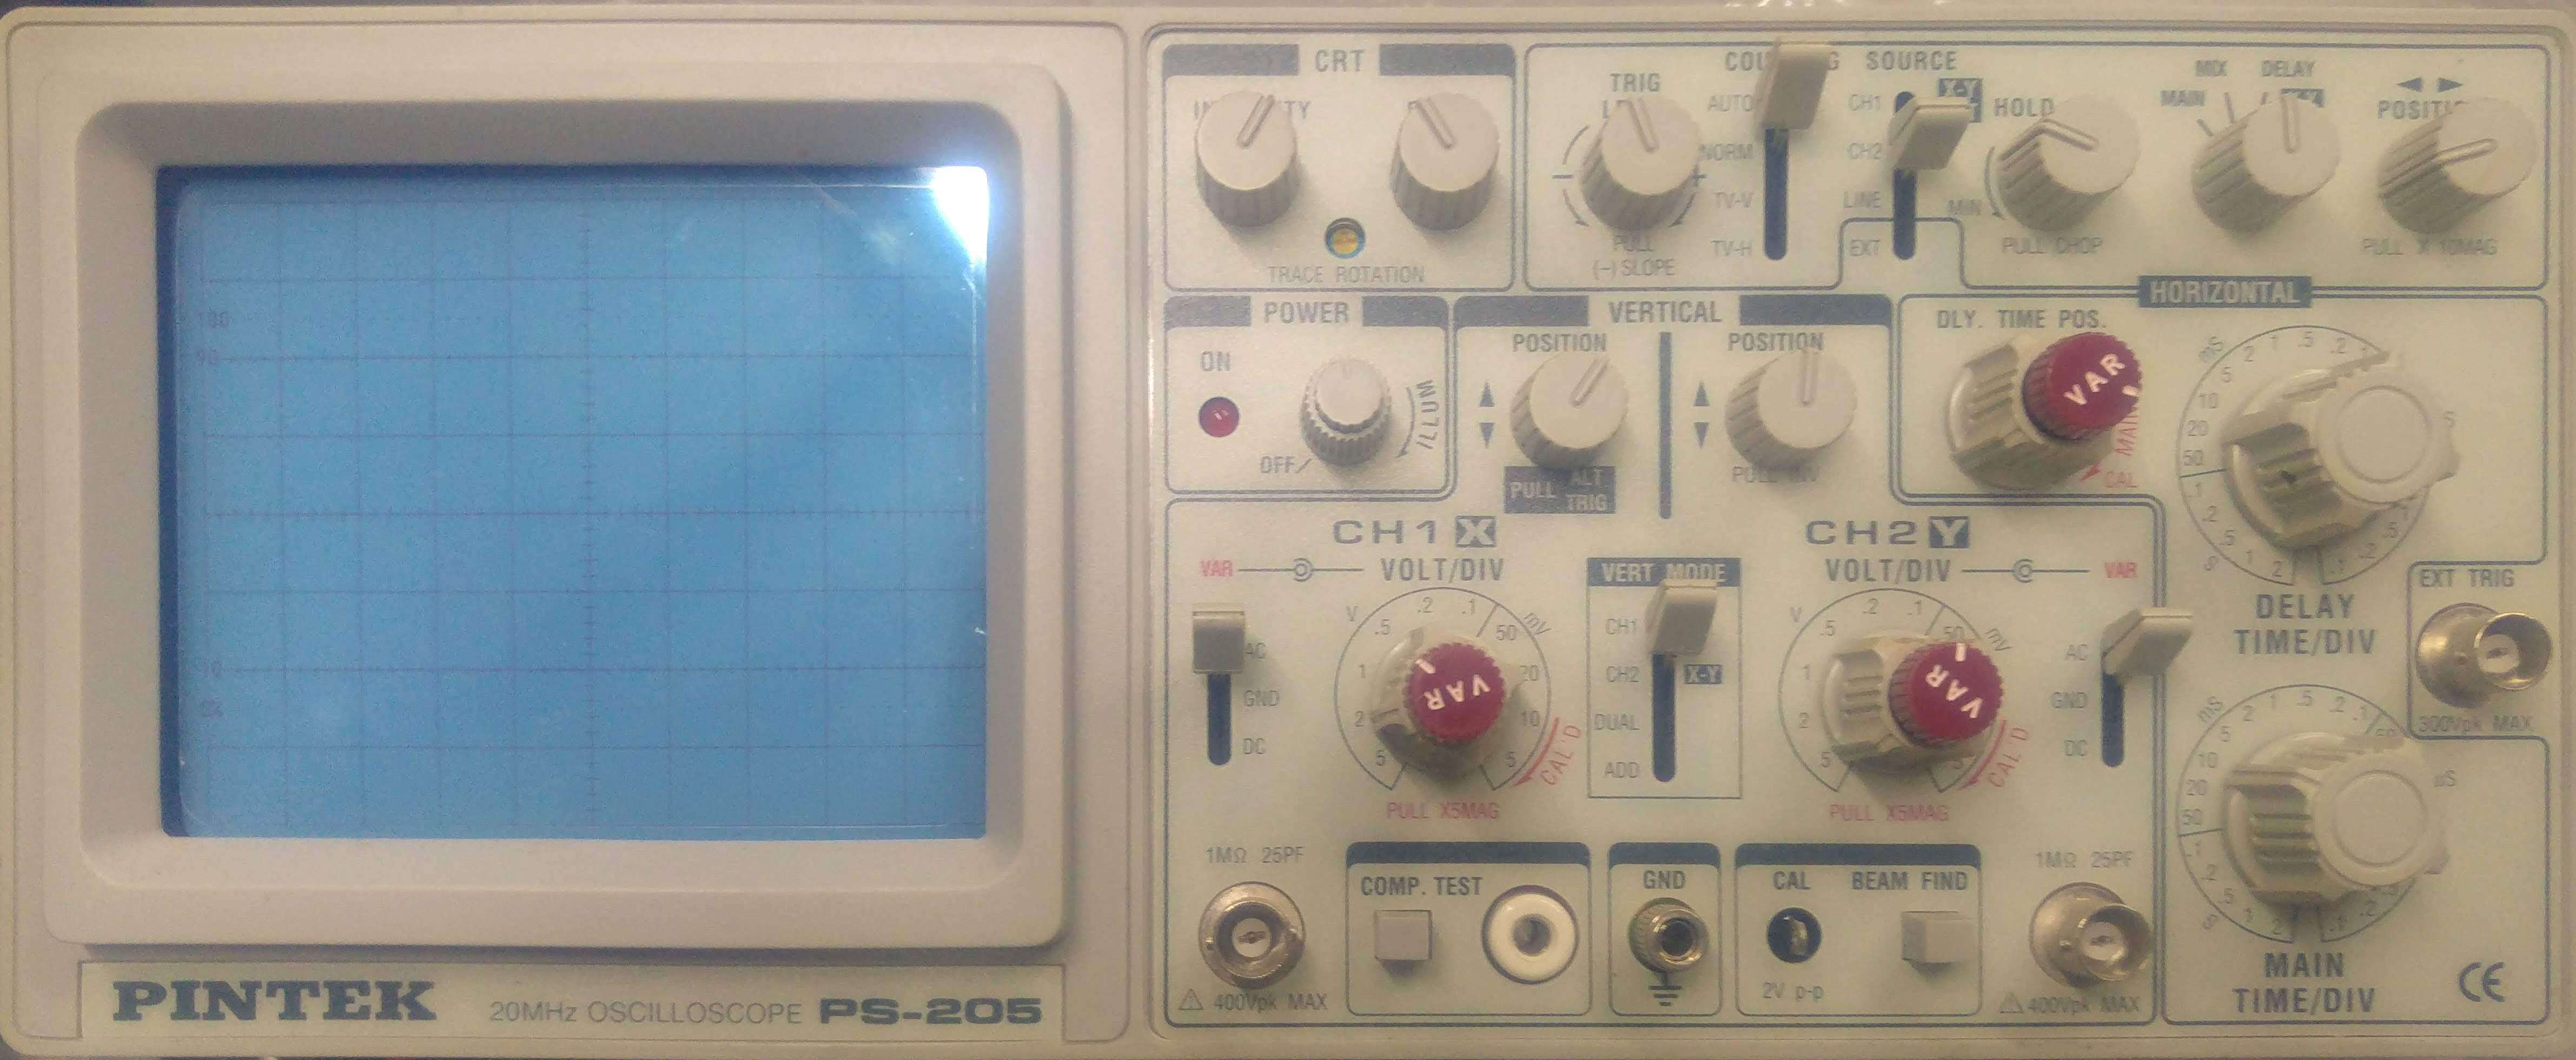
\includegraphics[width=\textwidth,height=\textheight,keepaspectratio]{images/fotos/osciloscopio2.jpg}
  \caption{Osciloscopio con pantalla CRT}
  \label{fig:osciloscopio_crt}
\end{figure}

\section{Comprobadores de tensión}
\subsection{Buscapolo}
\subsection{Medidor inductivo}
\section{Cofímetro o medidor de factor de potencia}

\begin{figure}[htbp]
  \centering
  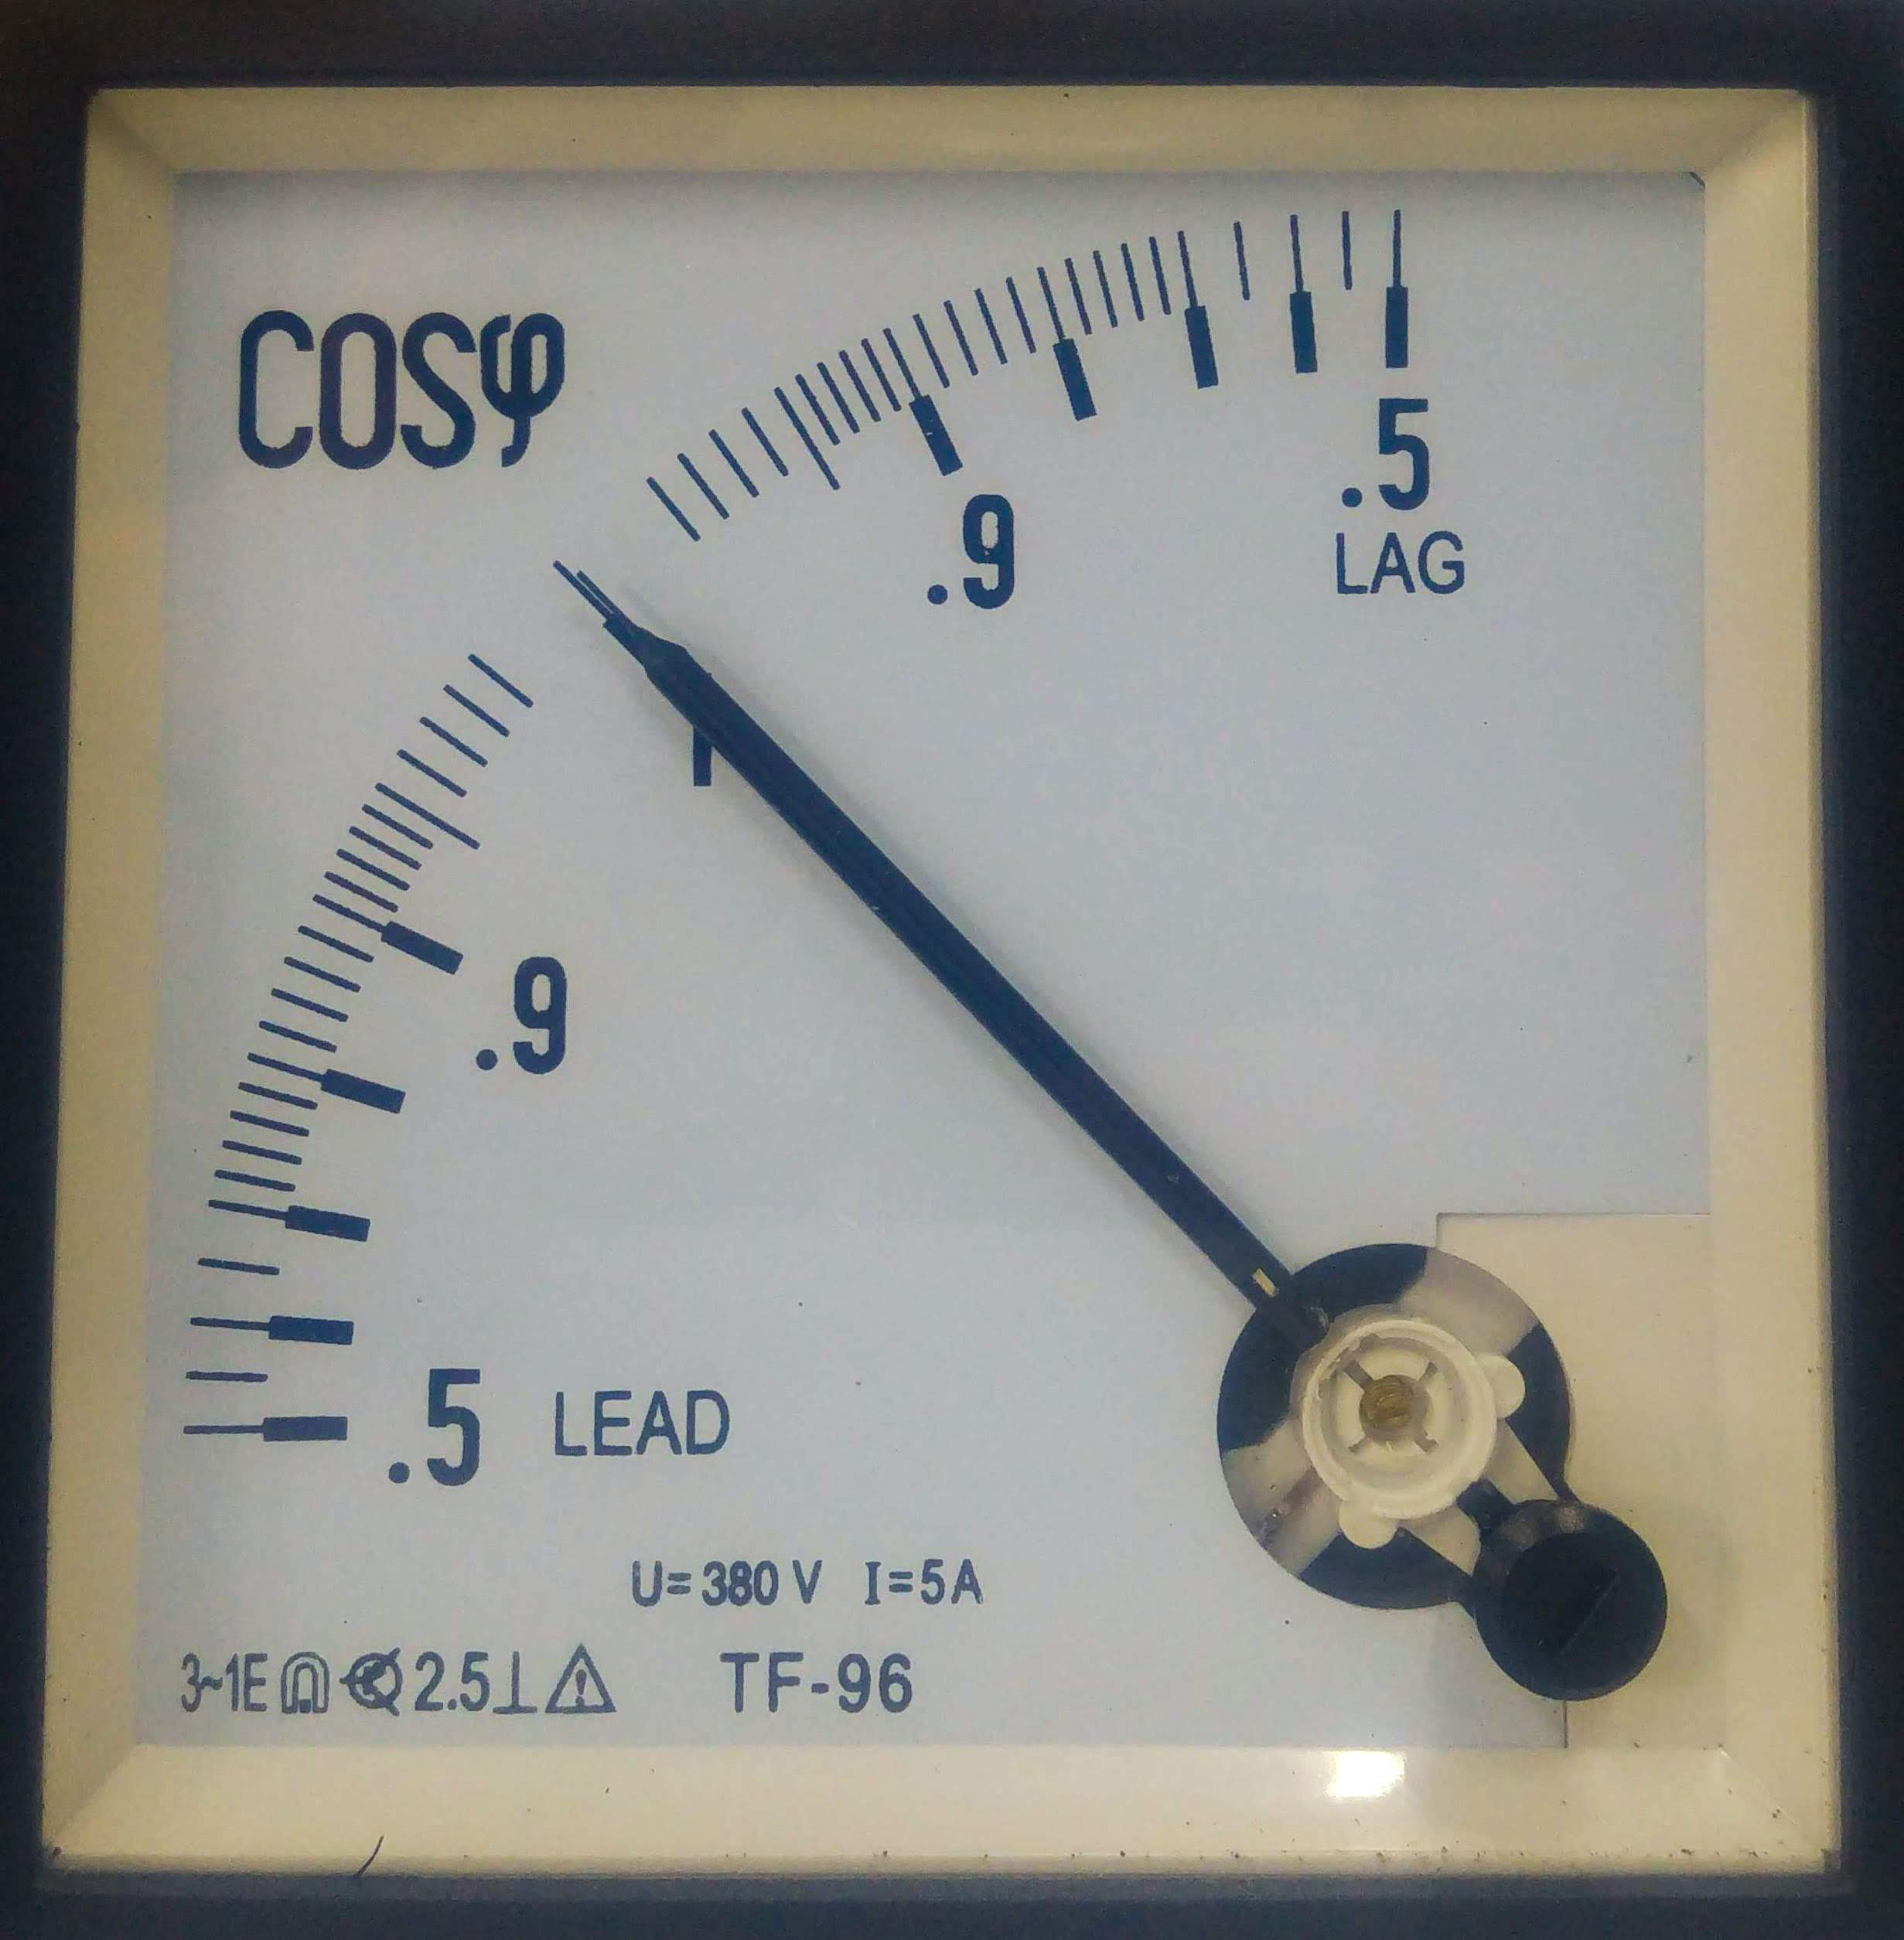
\includegraphics[width=0.5\textwidth,height=\textheight,keepaspectratio]{images/fotos/cofimetro.jpg}
  \caption{Medidor de factor de potencia (cofímetro) analógico}
  \label{fig:cofimetro}
\end{figure}

\section{Medidores de energía}

\subsection{Transformadores de corriente}
\section{Medidor de campo electromagnético}

\begin{figure}[htbp]
  \centering
  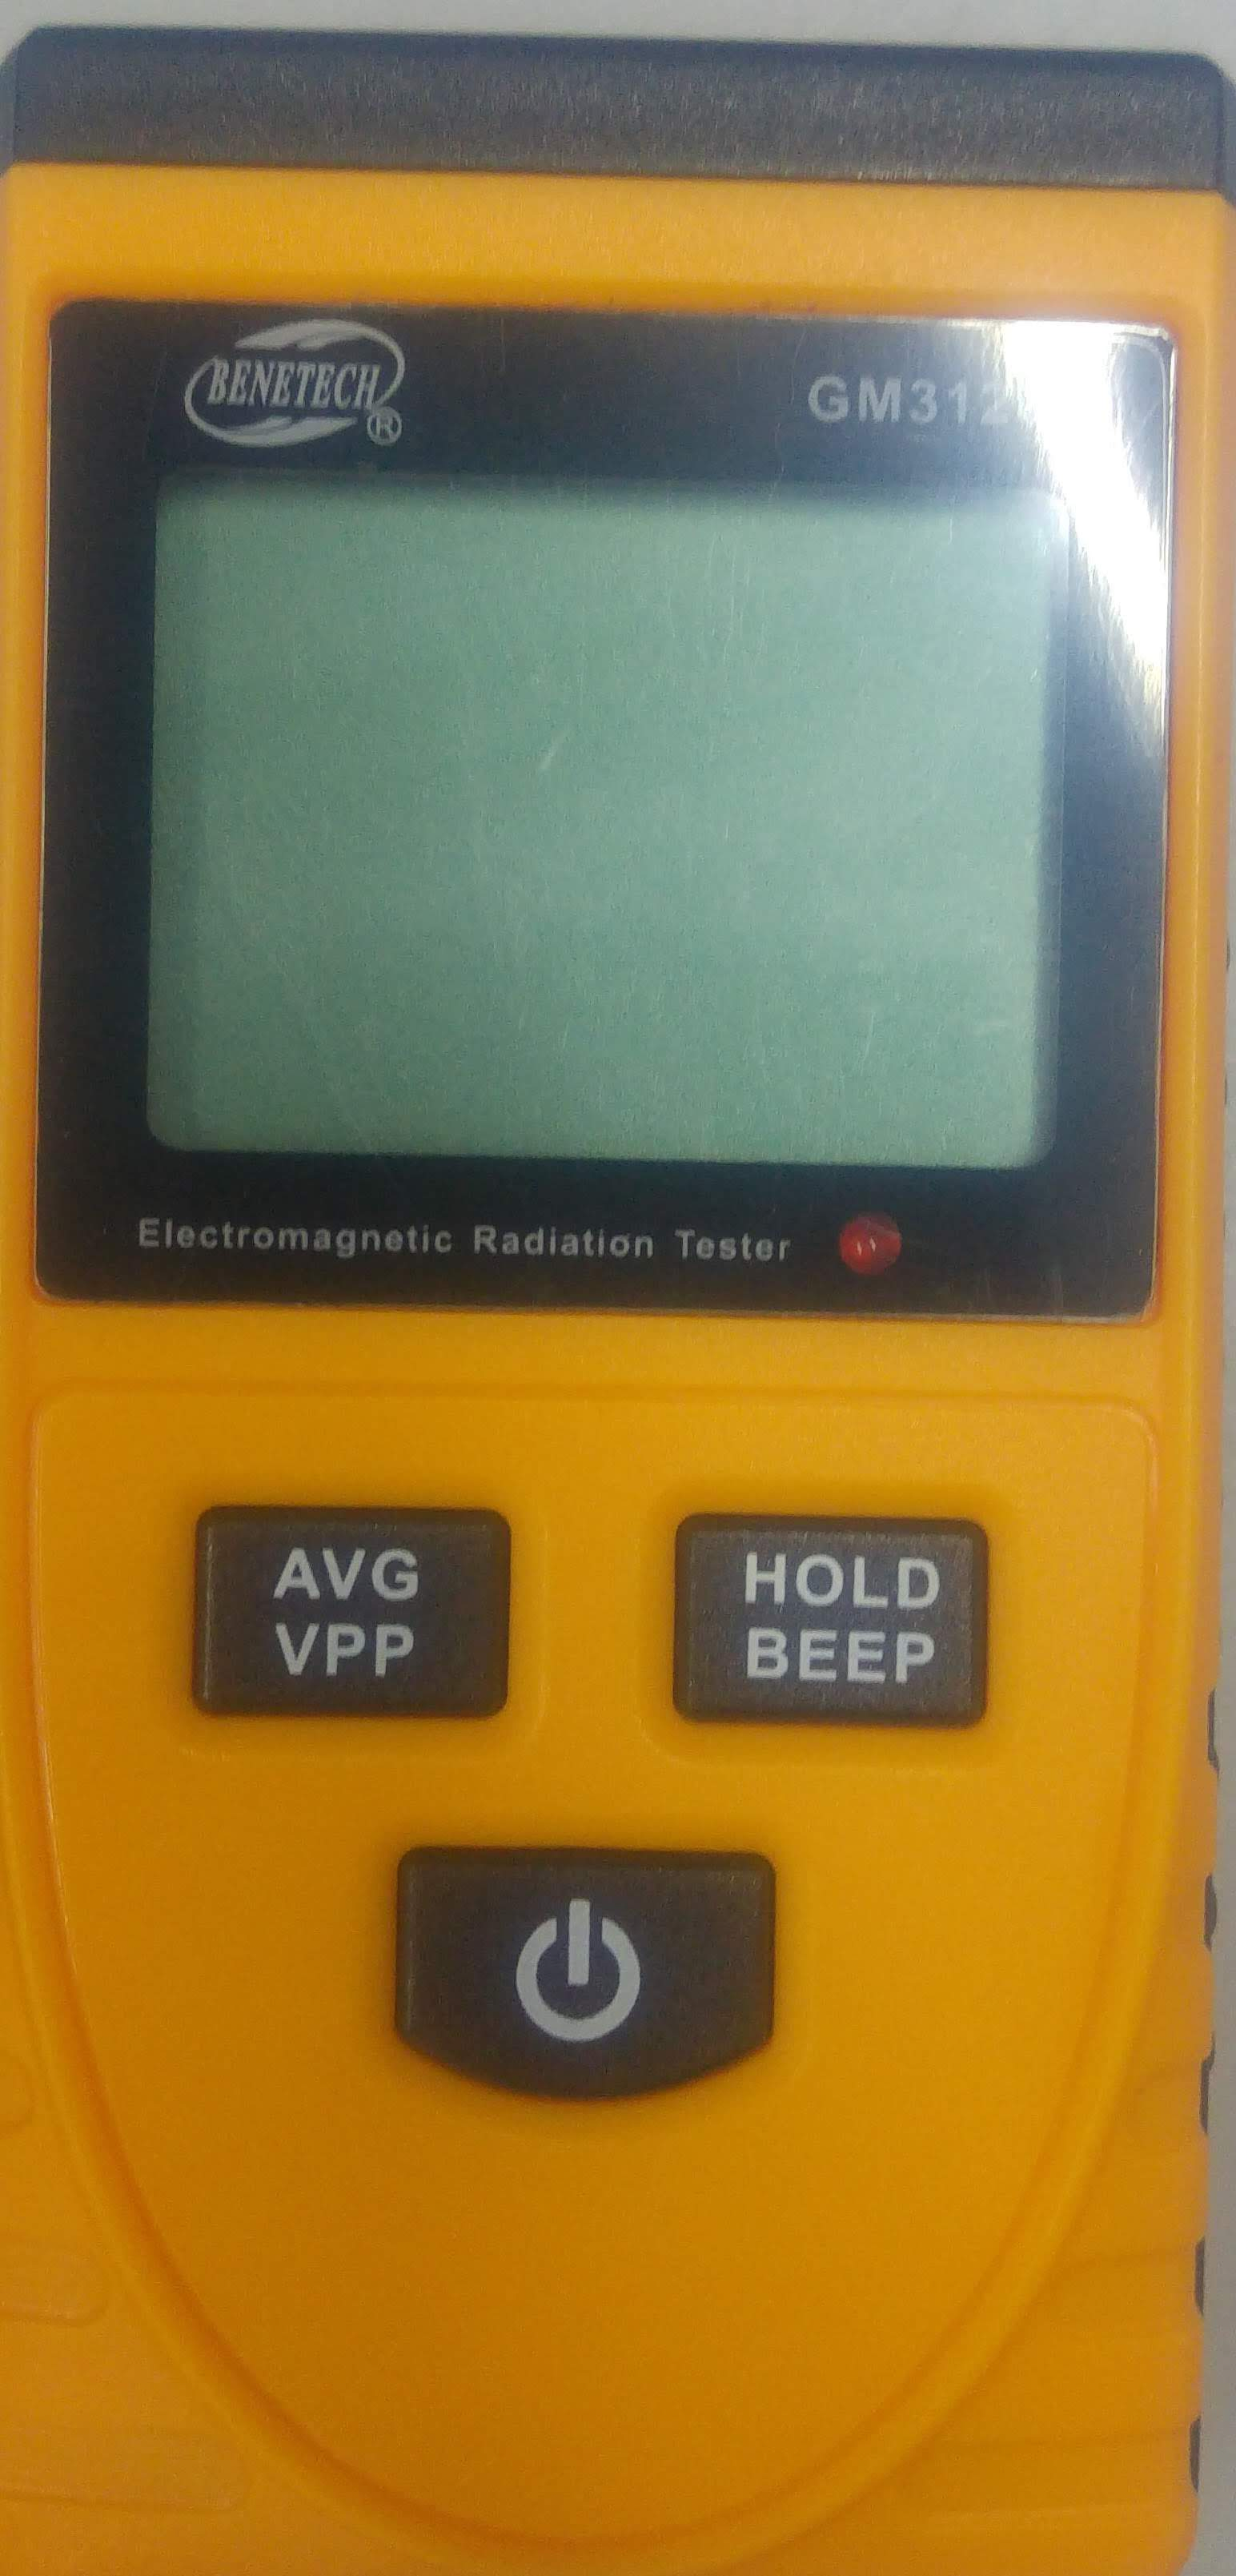
\includegraphics[width=0.3\textwidth,height=\textheight,keepaspectratio]{images/fotos/electromagnetico.jpg}
  \caption{Medidor de campo electromagnético}
  \label{fig:medidor_electromagnetico}
\end{figure}

\section{Milióhmetro}
\section{Generadores de funciones}

\begin{figure}[htbp]
  \centering
  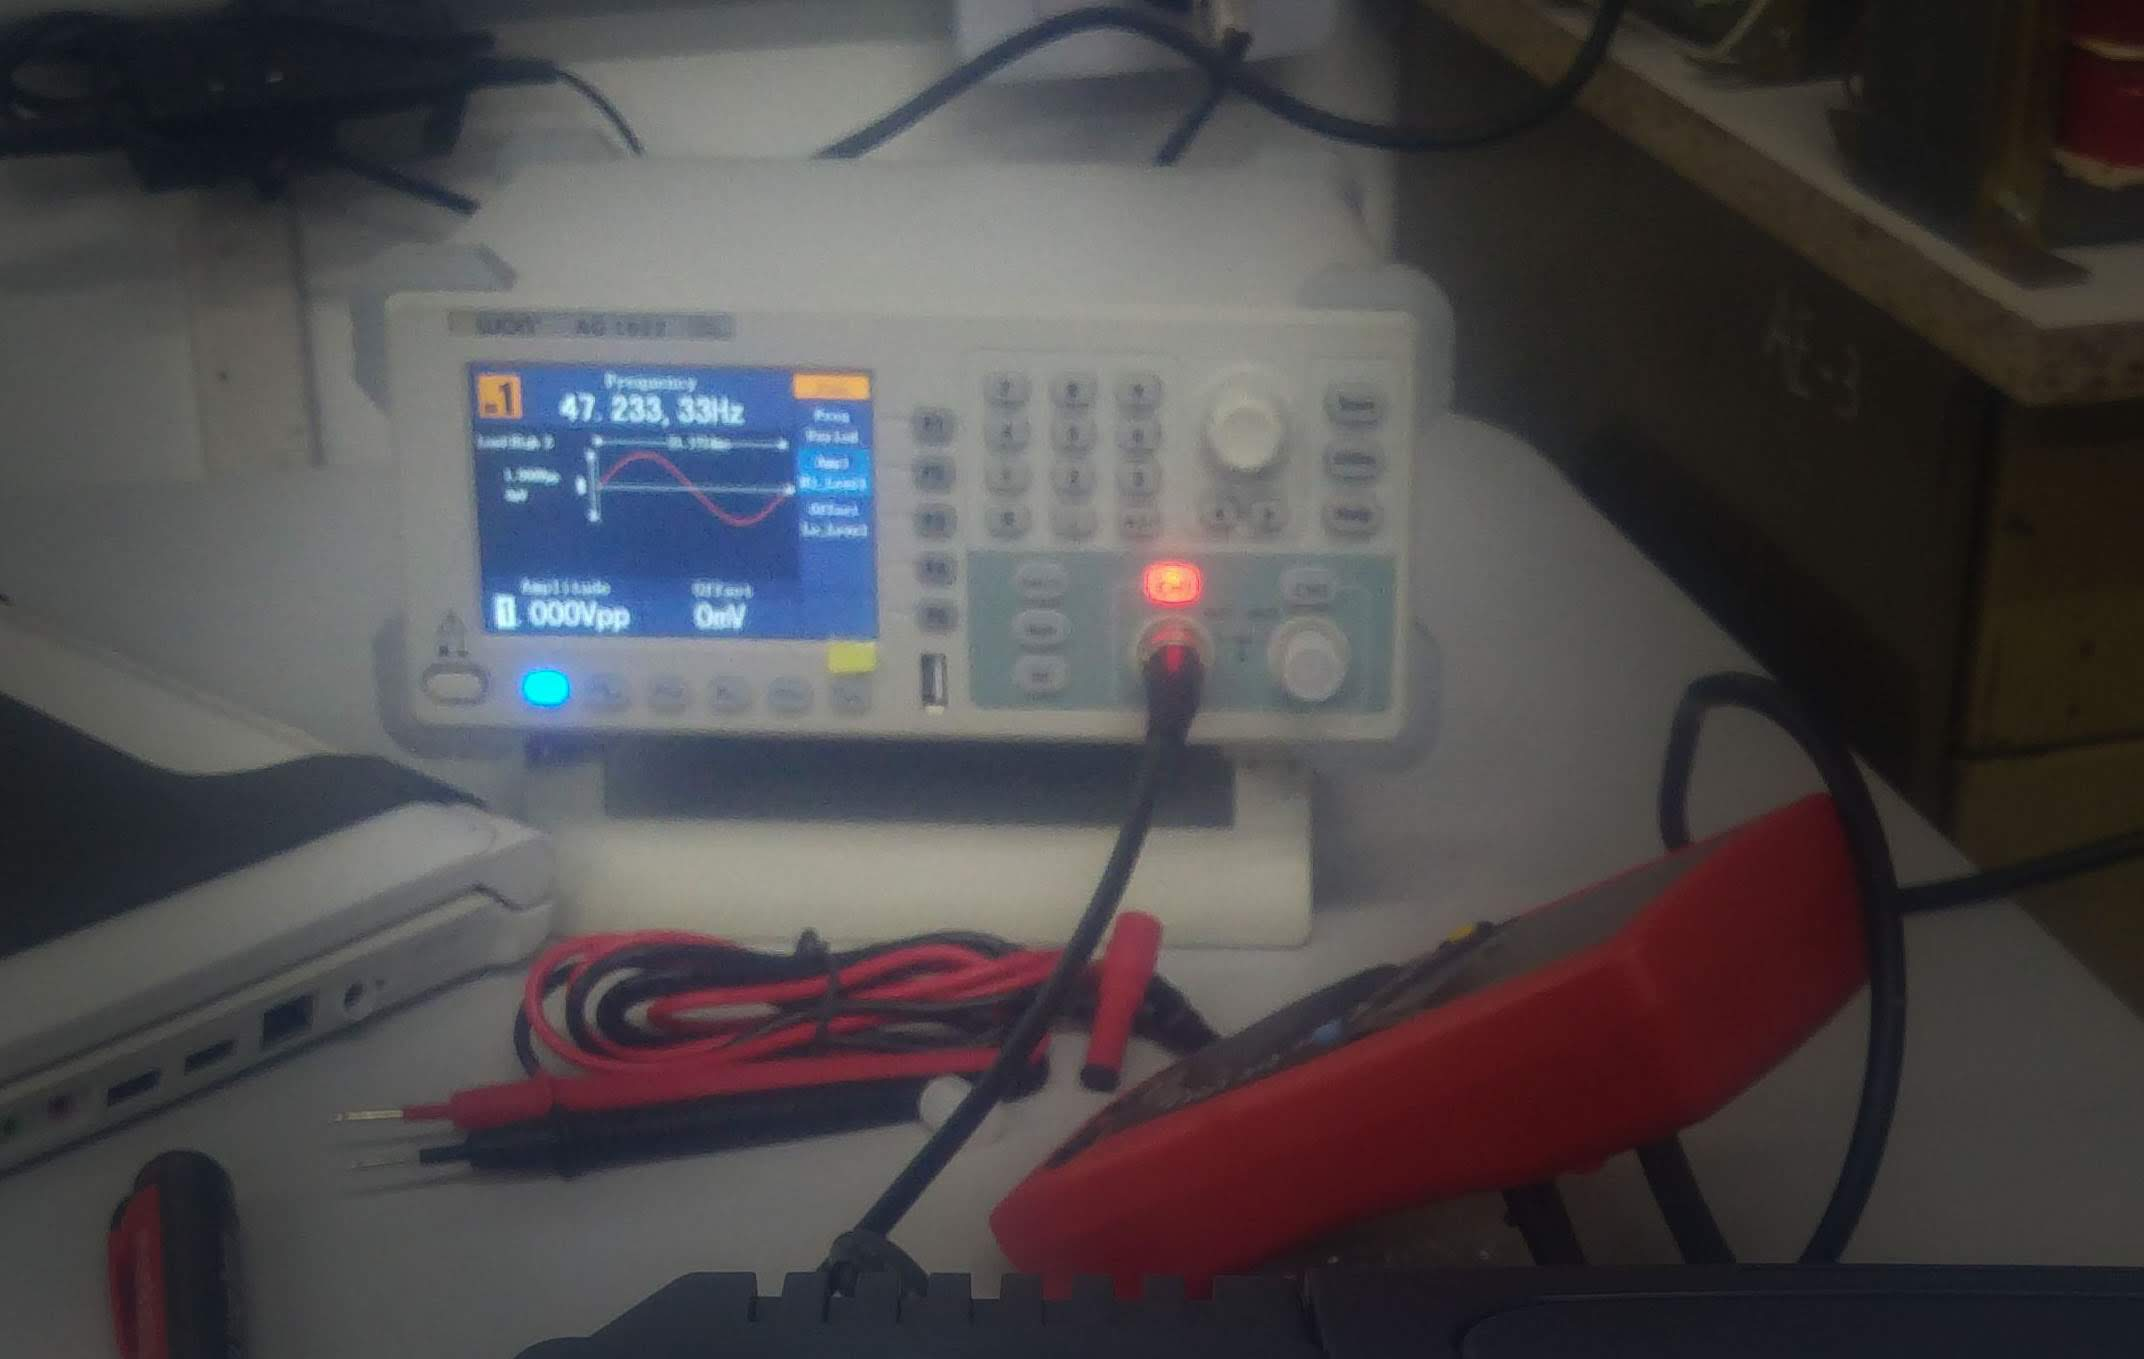
\includegraphics[width=\textwidth,height=\textheight,keepaspectratio]{images/fotos/generadordefunciones1.jpg}
  \caption{Generador de funciones}
  \label{fig:generador_funciones_1}
\end{figure}

\begin{figure}[htbp]
  \centering
  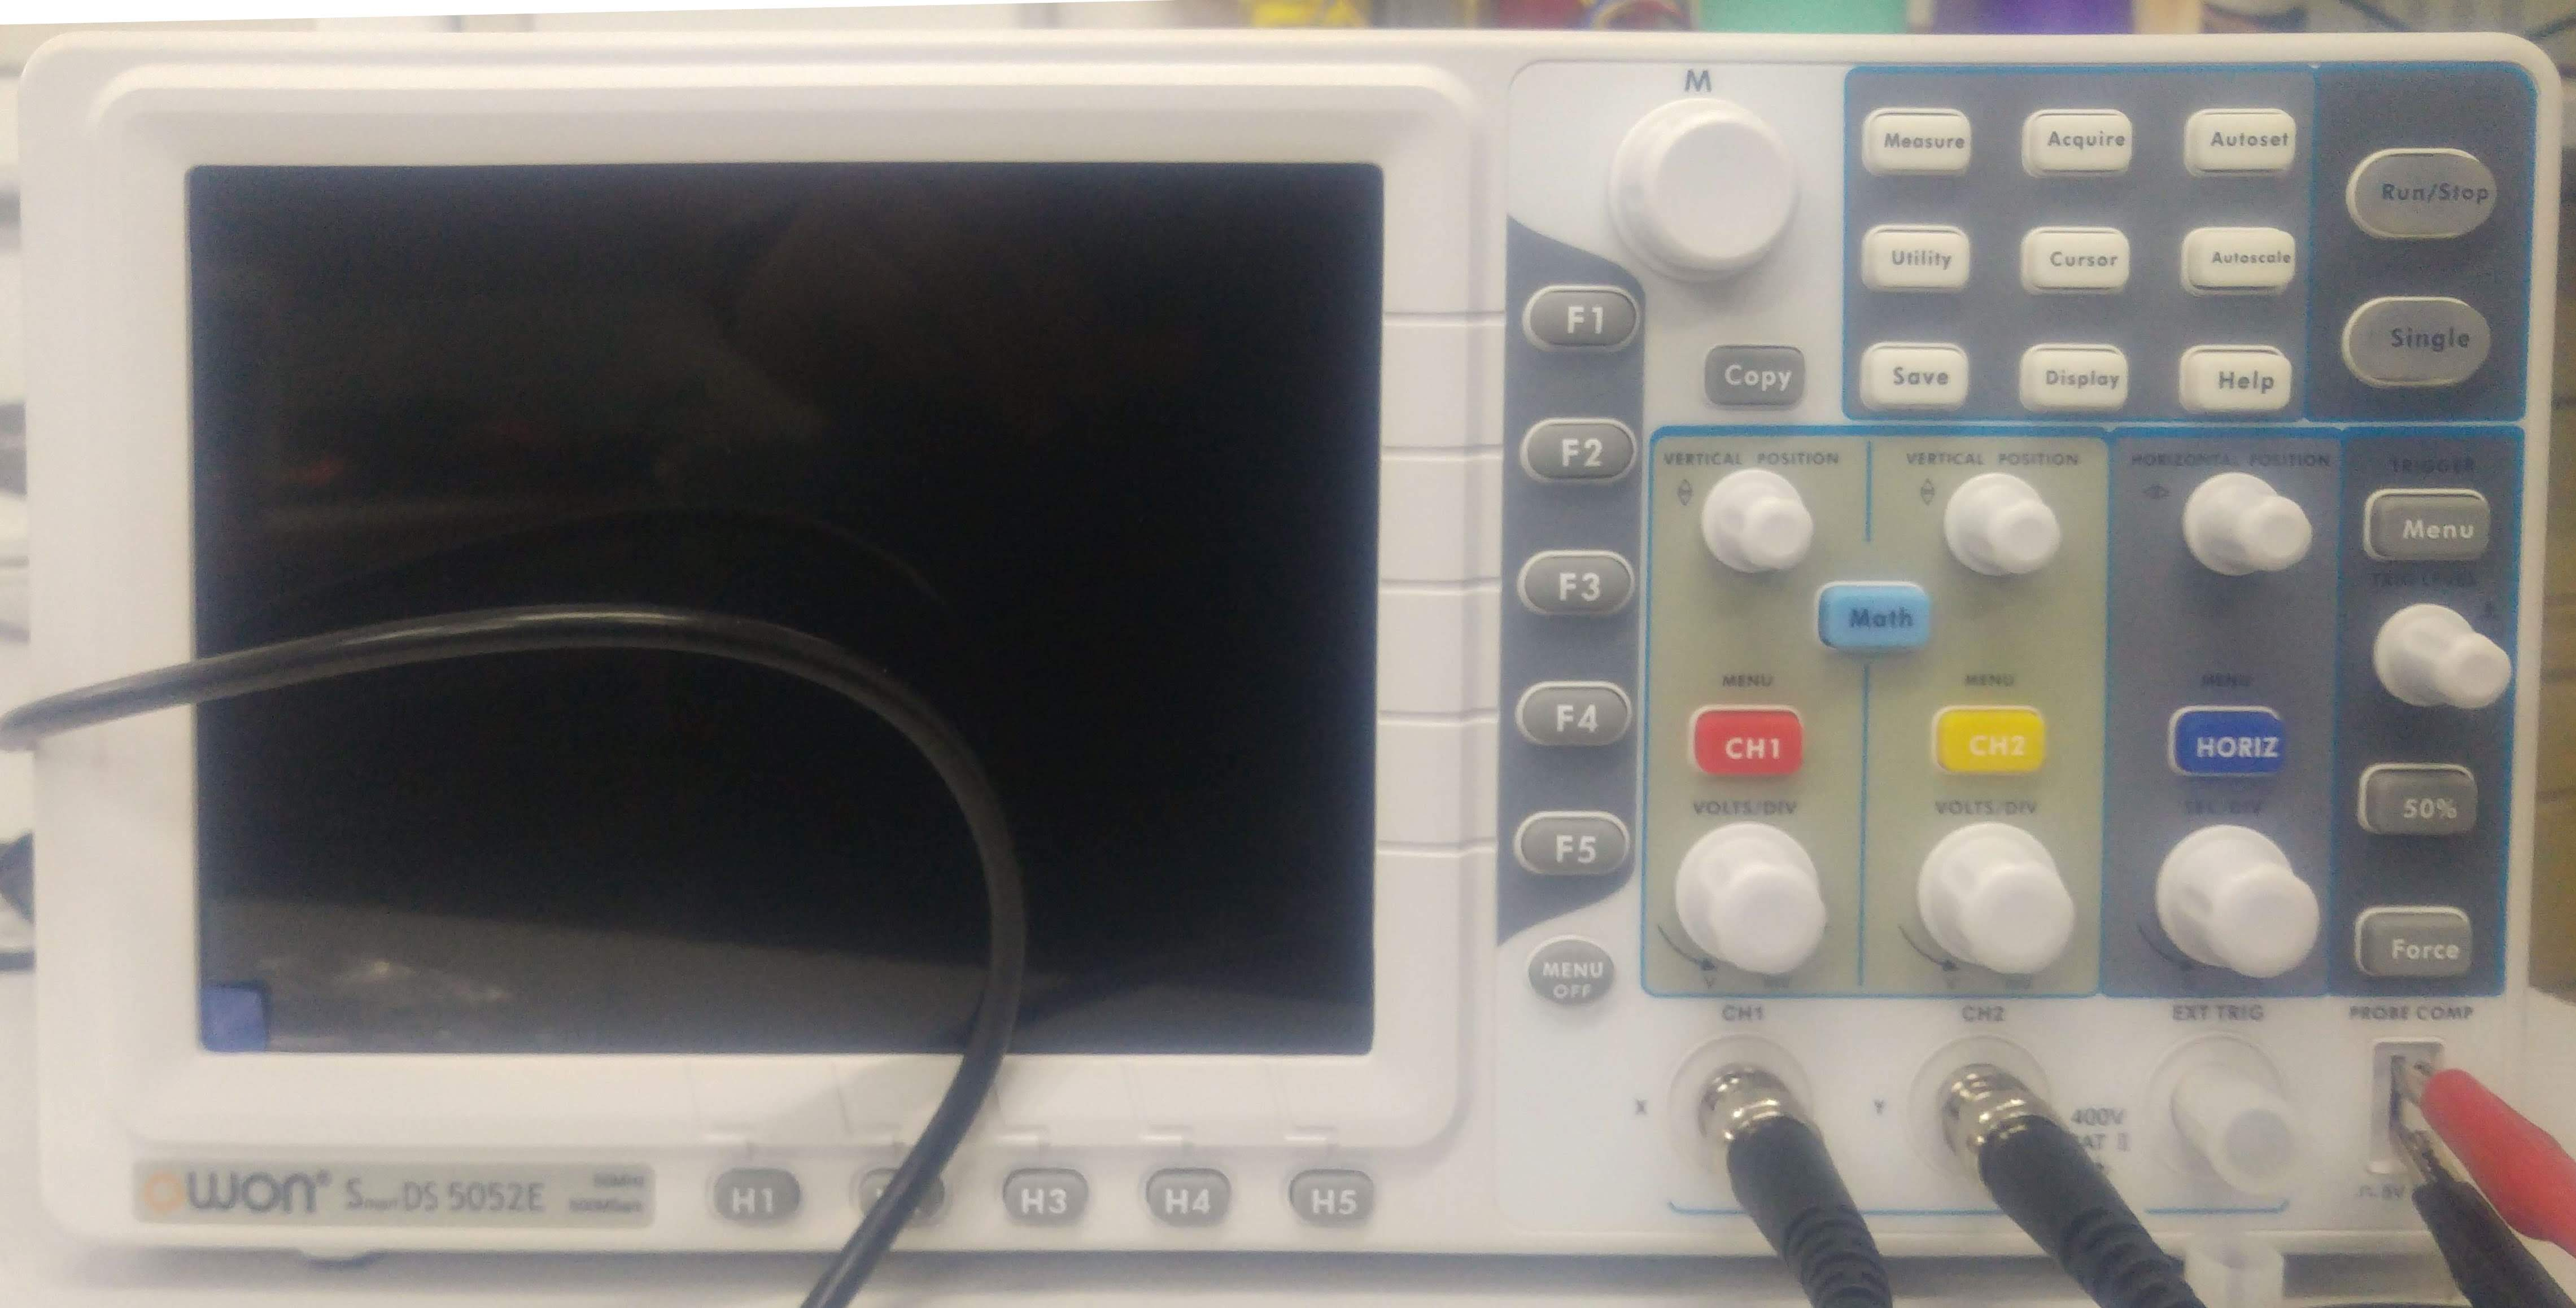
\includegraphics[width=\textwidth,height=\textheight,keepaspectratio]{images/fotos/generadordefunciones2.jpg}
  \caption{Generador de funciones}
  \label{fig:generador_funciones_2}
\end{figure}

\begin{figure}[htbp]
  \centering
  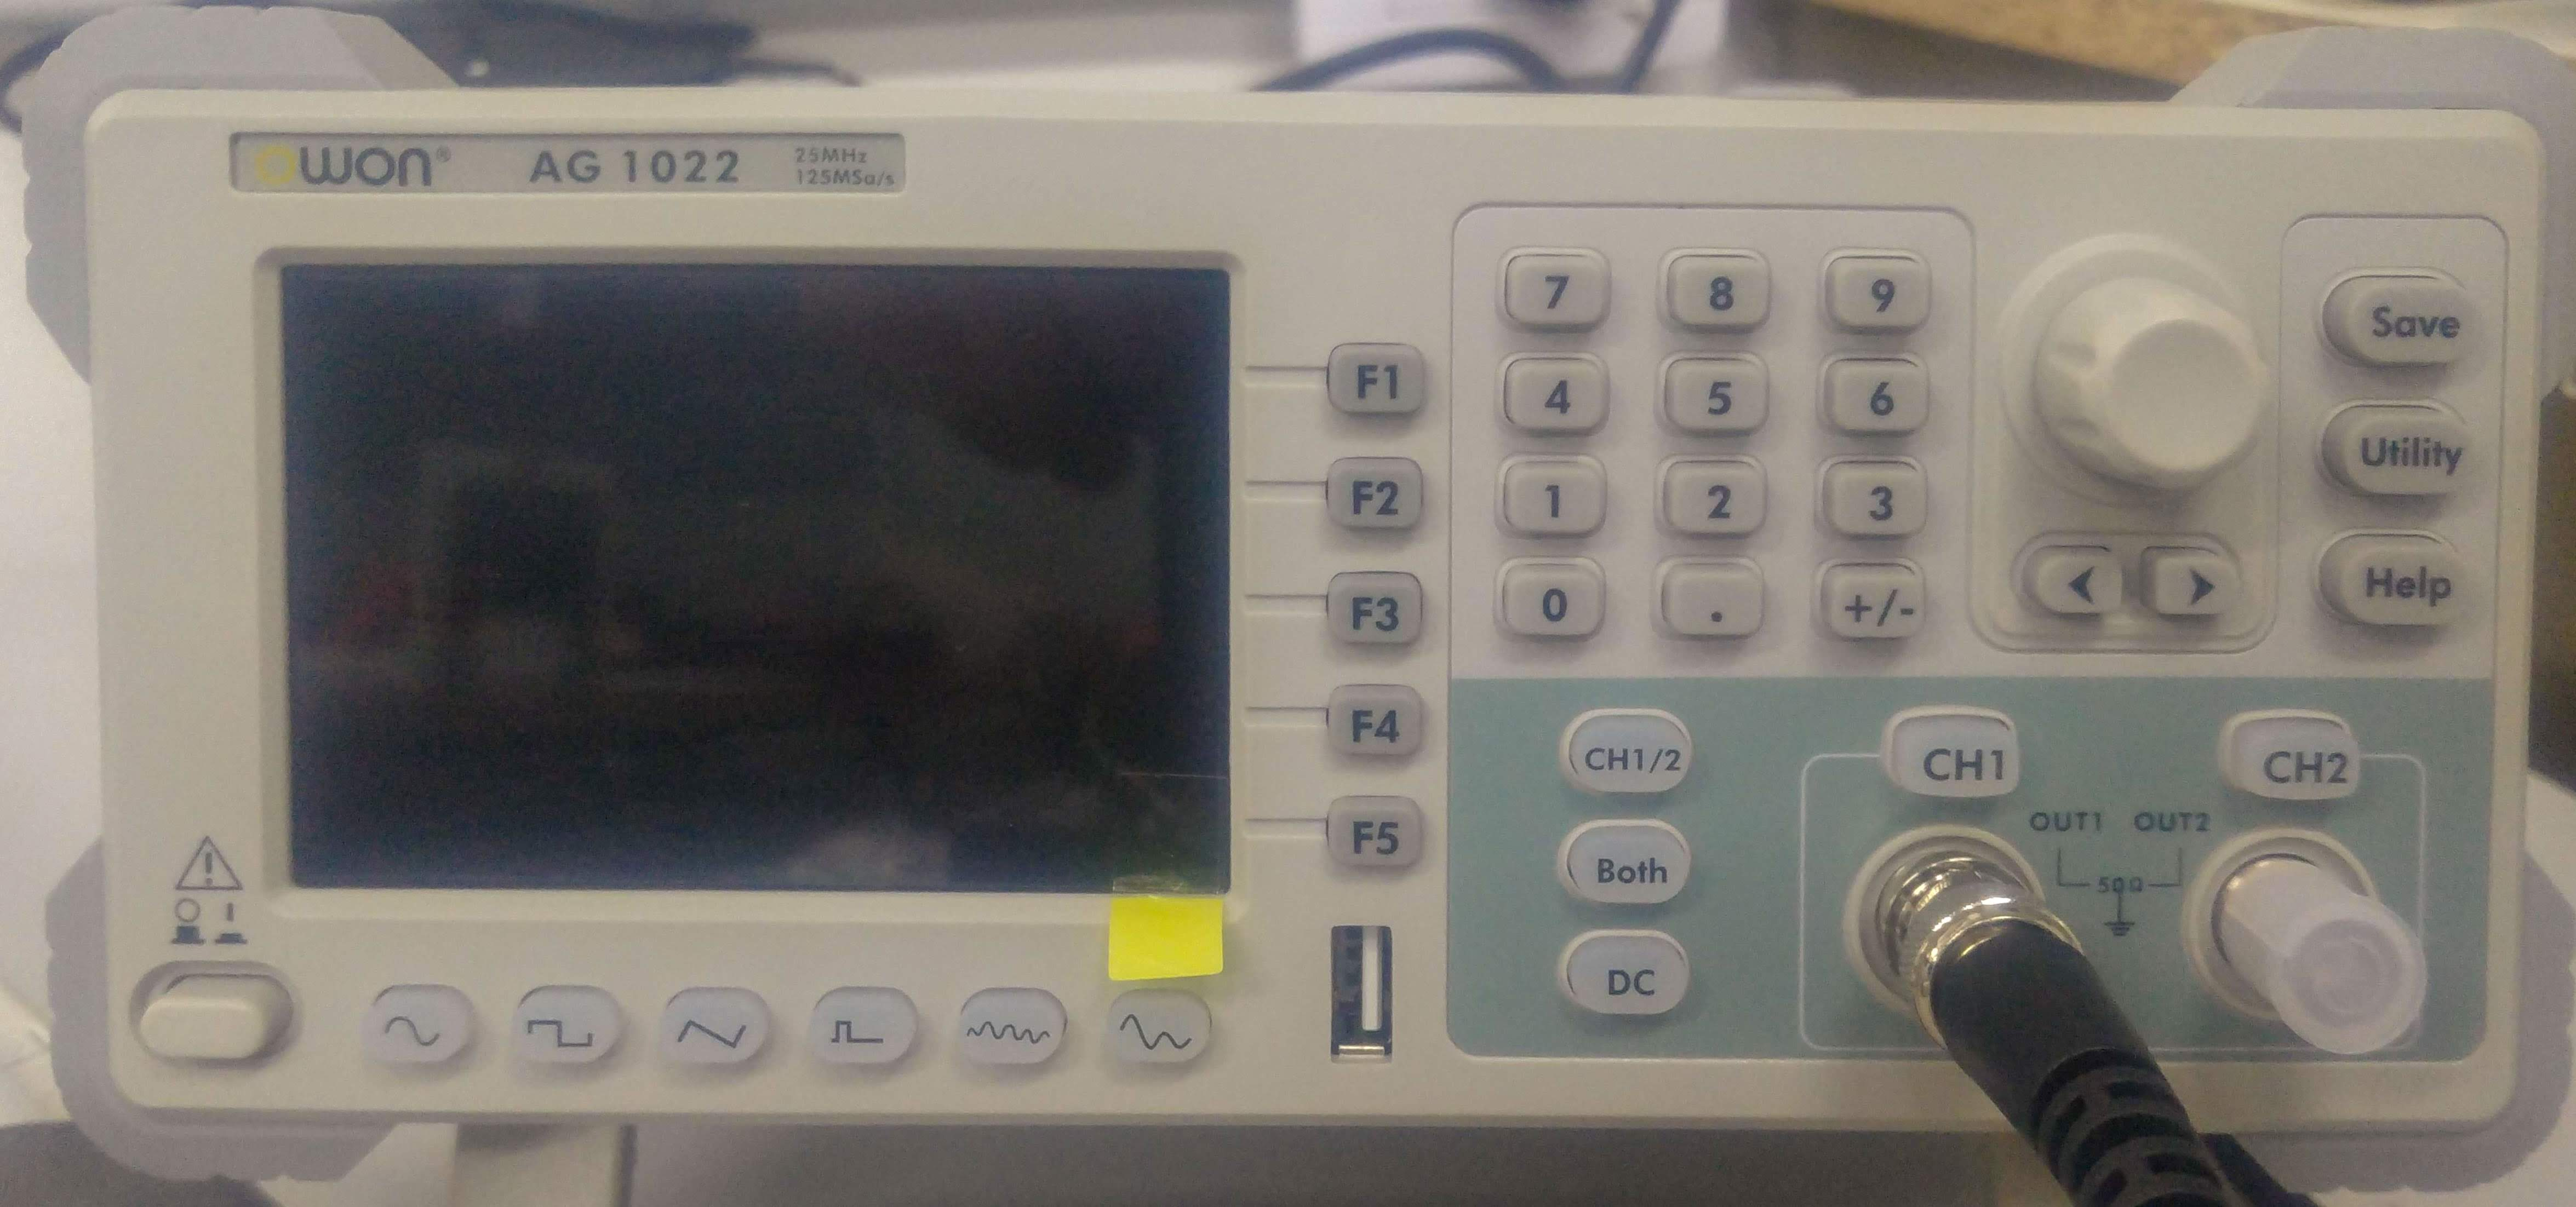
\includegraphics[width=\textwidth,height=\textheight,keepaspectratio]{images/fotos/generadordefunciones3.jpg}
  \caption{Generador de funciones}
  \label{fig:generador_funciones_3}
\end{figure}
